\documentclass{article}

% agents4science_2025 style package
\usepackage{agents4science_2025}

% Additional packages for the specific paper  
\usepackage{amsmath,amssymb}
\usepackage{siunitx}
\usepackage{algorithm}
\usepackage{algpseudocode}
\usepackage{enumitem}
\usepackage{adjustbox}
\usepackage{xspace}
\usepackage{tikz}
\usetikzlibrary{positioning} % for right=of syntax in TikZ diagrams
\usepackage{pgfplots}
\usepackage{tabularx}
\usepackage{array}
\usepackage{makecell}

\renewcommand\arraystretch{1.08}

\pgfplotsset{compat=1.18}

\sisetup{
  reset-text-series = false,
  text-series-to-math = true,
  reset-text-family = false,
  text-family-to-math = true,
  exponent-mode = scientific,
  round-mode = places,
  round-precision = 4,
  uncertainty-mode = separate,
  output-exponent-marker = \mathrm{e}
}
\DeclareSIUnit\dBm{dBm}
\newcommand{\nexact}[1]{#1}

\newcommand{\ie}{i.e.,\xspace}
\newcommand{\eg}{e.g.,\xspace}
\newcommand{\etal}{\textit{et al.}\xspace}

% Smaller mono for long command lines to reduce overfull boxes
\newcommand{\cmd}[1]{\par\noindent\begingroup\scriptsize\ttfamily\raggedright\sloppy #1\par\endgroup}

% Compact numeric rendering in running text (three significant figures).
\newcommand{\val}[1]{\num[round-mode=figures,round-precision=3]{#1}}

\hypersetup{
  pdftitle={CSS Threshold-Model BDD Monte Carlo with Distributed Coexistence Noise for Hollow-Core Fibers},
  pdfauthor={Agentic Research Group},
  pdfsubject={Single-file reproducible evaluation}
}

% ---------- In-document, runnable simulation (single source of truth; produces all numbers reported) ----------
% Use a jobname-derived artifact filename to avoid literal filenames in the source/PDF.
% IMPORTANT: write a .py file explicitly to ensure robust shell-escape execution across TeX distributions.
\begin{filecontents*}[overwrite]{\jobname-artifact.py}
#!/usr/bin/env python3
# -*- coding: utf-8 -*-
"""
Reproducible Monte Carlo used for the results reported in the paper.

Authoritative model (Model 2):
  - Physics-driven mapping from HCF coexistence parameters to asymmetric Pauli
    error probabilities using distributed integrals along the span:
      SpRS ~ c_R * ∫ P(z) dz,  FWM ~ c_F * Δλ * ∫ P(z)^2 dz,
    with P(z)=P0*exp(-alpha*z), alpha = kappa * alpha_dB (nepers/km).
  - Temporal correlation via a two-state Markov-modulated Bernoulli process (MMBP)
    with persistence rho (Gilbert--Elliott style). The "bad" state's error prob.
    is scaled by a user parameter beta (default 2.0), clipped to 1.
  - Block failure under bounded-distance decoding (BDD): fail if wX>t or wZ>t.
  - 95% Wilson intervals; optional report of expected run length 1/(1-rho).

Outputs CSV with point estimates, 95% Wilson confidence intervals, raw counts,
and throughput measurements.

Optional: --emit-tex-macros to print TeX \\newcommand definitions for all macros
used by the paper (no CSV). This enables compile-time macro regeneration when
shell-escape is available; otherwise the paper uses static fallback macros.

Additional optional PGFPlots emitters for full figure traceability (all figures in this paper):
  --emit-pgf-rho         Emit coordinates for the rho sweep (P_L vs rho) with symmetric Wilson half-widths
  --emit-pgf-runlen      Emit analytic expected run length points vs rho (y = 1/(1-rho))
  --emit-pgf-length      Emit coordinates for length sweep (L vs P_L)
  --emit-pgf-power       Emit coordinates for power sweep (P_cl vs P_L)
  --emit-pgf-sep         Emit coordinates for separation sweep (Δλ vs P_L)
  --emit-pgf-eta         Emit coordinates for asymmetry sweep (eta_px vs P_L)

Python: 3.8+ (stdlib only)
"""

import argparse, math, random, sys, time, platform
from typing import List, Tuple, Dict

def set_seed(seed: int) -> None:
    random.seed(seed)

def hcf_noise_model(length_km: float,
                    classical_power_dBm: float,
                    wavelength_separation_nm: float,
                    raman_coeff: float = 0.025,
                    fwm_coeff: float = 1e-4,
                    attenuation_db_per_km: float = 0.25,
                    eta_px: float = 0.3,
                    atten_kappa: float = 0.1) -> Tuple[float,float,float,float,float]:
    """Effective physics-inspired mapping using distributed-noise integrals."""
    P0 = 10 ** ((classical_power_dBm - 30) / 10.0)  # W
    alpha = attenuation_db_per_km * atten_kappa     # nepers/km
    if alpha <= 0:
        alpha = 1e-12
    I1 = (P0/alpha) * (1.0 - math.exp(-alpha * length_km))
    I2 = (P0*P0/(2.0*alpha)) * (1.0 - math.exp(-2.0*alpha * length_km))
    sprs = raman_coeff * I1
    fwm  = fwm_coeff  * wavelength_separation_nm * I2
    tau = sprs + fwm
    pz = 1.0 - math.exp(-tau)
    px = eta_px * pz
    return px, pz, sprs, fwm, alpha

def markov_states(rho: float, n: int) -> List[int]:
    """Generate hidden states for a symmetric two-state MMBP with persistence rho."""
    state = 1 if random.random() < 0.5 else 0
    out = [0]*n
    for i in range(n):
        out[i] = state
        if random.random() > rho:
            state ^= 1
    return out

def markov_bits(p_base: float, rho: float, n: int, beta: float) -> List[int]:
    """Two-state symmetric MMBP: low-noise: p_base; high-noise: min(1, beta*p_base)."""
    states = markov_states(rho, n)
    out = [0]*n
    hi = min(1.0, beta*p_base)
    for i, s in enumerate(states):
        p = p_base if s == 0 else hi
        out[i] = 1 if random.random() < p else 0
    return out

def bdd_block_fail_model2(n: int, t: int, px: float, pz: float, rho: float, trials: int,
                          beta: float = 2.0,
                          shared_state: bool=False) -> Tuple[int,int]:
    """Return (failures, trials) under Model 2 with BDD threshold criterion."""
    fails = 0
    for _ in range(trials):
        if shared_state:
            states = markov_states(rho, n)
            hiX = min(1.0, beta*px)
            hiZ = min(1.0, beta*pz)
            x = [1 if random.random() < (px if s == 0 else hiX) else 0 for s in states]
            z = [1 if random.random() < (pz if s == 0 else hiZ) else 0 for s in states]
        else:
            x = markov_bits(px, rho, n, beta)
            z = markov_bits(pz, rho, n, beta)
        if sum(x) > t or sum(z) > t:
            fails += 1
    return fails, trials

def depolarizing_trial(n: int, t: int, p: float) -> bool:
    """Single codeword trial under depolarizing channel with error prob p."""
    wx = wz = 0
    for _ in range(n):
        r = random.random()
        if r < p/3.0:            # X
            wx += 1
        elif r < 2*p/3.0:        # Y
            wx += 1; wz += 1
        elif r < p:              # Z
            wz += 1
    return (wx > t) or (wz > t)

def bdd_block_fail_depol(n: int, t: int, p: float, trials: int) -> Tuple[int,int]:
    """Return (failures, trials) under i.i.d. depolarizing channel."""
    fails = 0
    for _ in range(trials):
        if depolarizing_trial(n, t, p):
            fails += 1
    return fails, trials

def wilson_interval(k: int, n: int) -> Tuple[float,float,float]:
    """Wilson score interval for binomial proportion (95%)."""
    if n == 0:
        return (0.0, 0.0, 0.0)
    from math import sqrt
    z = 1.959963984540054 # 95%
    phat = k/n
    denom = 1 + z*z/n
    center = (phat + z*z/(2*n)) / denom
    half = (z/denom) * sqrt(phat*(1-phat)/n + z*z/(4*n*n))
    lo = max(0.0, center-half)
    hi = min(1.0, center+half)
    return phat, lo, hi

def f8(x: float) -> str:
    return f"{x:.8e}"

def emit_tex_macros(args,
                    px_base, pz_base,
                    main_res,
                    rho_points: Dict[float,Tuple[float,float,float,int]],
                    length_points: Dict[float,Tuple[float,float,Tuple[float,float,float,int]]],
                    power_points: Dict[float,Tuple[float,float,Tuple[float,float,float,int]]],
                    sep_points: Dict[float,Tuple[float,float,Tuple[float,float,float,int],float]],
                    eta_points: Dict[float,Tuple[float,Tuple[float,float,float,int]]]):
    """Print TeX \\newcommand definitions matching the paper macros (self-contained traceability)."""
    # Baseline params
    print(f"\\newcommand{{\\simL}}{{{int(args.L)}}}")
    print(f"\\newcommand{{\\simpcl}}{{{int(args.pcl)}}}")
    print(f"\\newcommand{{\\simsep}}{{{args.sep_nm}}}")
    print(f"\\newcommand{{\\simeta}}{{{args.eta_px}}}")
    print(f"\\newcommand{{\\simn}}{{{args.n}}}")
    print(f"\\newcommand{{\\simt}}{{{args.t}}}")
    print(f"\\newcommand{{\\simtrials}}{{{args.trials_bdd}}}")
    print(f"\\newcommand{{\\simseed}}{{{args.seed}}}")
    print(f"\\newcommand{{\\simpz}}{{{f8(pz_base)}}}")
    print(f"\\newcommand{{\\simpx}}{{{f8(px_base)}}}")
    # Derived baselines
    p_eff_sum = 0.5*(min(1.0, args.beta*px_base)+px_base) + 0.5*(min(1.0, args.beta*pz_base)+pz_base)
    print(f"\\newcommand{{\\simpesum}}{{{f8(p_eff_sum)}}}")
    # Main result (and timing)
    ph, lo, hi, k = main_res
    print(f"\\newcommand{{\\simrhoB}}{{{args.rho:.2f}}}")
    print(f"\\newcommand{{\\simpLB}}{{{f8(ph)}}}")
    print(f"\\newcommand{{\\simpLBlo}}{{{f8(lo)}}}")
    print(f"\\newcommand{{\\simpLBhi}}{{{f8(hi)}}}")
    print(f"\\newcommand{{\\simkB}}{{{k}}}")
    if ph > 0:
        rel_half = max(ph-lo, hi-ph)/ph
        print(f"\\newcommand{{\\simRelHalfWidthMain}}{{{100.0*rel_half:.1f}\\%}}")
    # Rho sweep
    order = [(0.00,"D"),(0.30,"A"),(0.60,"B"),(0.85,"C"),(0.95,"E")]
    for r, tag in order:
        ph, lo, hi, k = rho_points[r]
        print(f"\\newcommand{{\\simrho{tag}}}{{{r:.2f}}}")
        print(f"\\newcommand{{\\simpL{tag}}}{{{f8(ph)}}}")
        print(f"\\newcommand{{\\simpL{tag}lo}}{{{f8(lo)}}}")
        print(f"\\newcommand{{\\simpL{tag}hi}}{{{f8(hi)}}}")
        print(f"\\newcommand{{\\simk{tag}}}{{{k}}}")
    # Length sweep (selected)
    for L,label in [(50.0,"Lfa"),(150.0,"Lfb")]:
        pz, px, res = length_points[L]
        ph, lo, hi, k = res
        print(f"\\newcommand{{\\sim{label}}}{{{int(L)}}}")
        print(f"\\newcommand{{\\simpz{label}}}{{{f8(pz)}}}")
        print(f"\\newcommand{{\\simpx{label}}}{{{f8(px)}}}")
        print(f"\\newcommand{{\\simpL{label}}}{{{f8(ph)}}}")
        print(f"\\newcommand{{\\simpL{label}lo}}{{{f8(lo)}}}")
        print(f"\\newcommand{{\\simpL{label}hi}}{{{f8(hi)}}}")
        print(f"\\newcommand{{\\simk{label}}}{{{k}}}")
    # Power sweep (selected)
    for P,label in [(0.0,"PclA"),(5.0,"PclB")]:
        pz, px, res = power_points[P]
        ph, lo, hi, k = res
        print(f"\\newcommand{{\\simpcl{label[-1]}}}{{{int(P)}}}")
        print(f"\\newcommand{{\\simpz{label}}}{{{f8(pz)}}}")
        print(f"\\newcommand{{\\simpx{label}}}{{{f8(px)}}}")
        print(f"\\newcommand{{\\simpL{label}}}{{{f8(ph)}}}")
        print(f"\\newcommand{{\\simpL{label}lo}}{{{f8(lo)}}}")
        print(f"\\newcommand{{\\simpL{label}hi}}{{{f8(hi)}}}")
        print(f"\\newcommand{{\\simk{label}}}{{{k}}}")
    # Separation sweep, include FWM terms and fraction for main point
    _, _, sprs_base, fwm_base, _ = hcf_noise_model(args.L, args.pcl, args.sep_nm,
                                                   eta_px=args.eta_px, atten_kappa=args.atten_kappa)
    if sprs_base > 0:
        frac = 100.0*(fwm_base/sprs_base)
        print(f"\\newcommand{{\\simFWMFrac}}{{{frac:.1e}\\%}}")
    for S,label in [(3.2,"SepA"),(12.8,"SepB")]:
        pz, px, res, fwm = sep_points[S]
        ph, lo, hi, k = res
        print(f"\\newcommand{{\\simsep{label[-1]}}}{{{S}}}")
        print(f"\\newcommand{{\\simpz{label}}}{{{f8(pz)}}}")
        print(f"\\newcommand{{\\simpx{label}}}{{{f8(px)}}}")
        print(f"\\newcommand{{\\simpL{label}}}{{{f8(ph)}}}")
        print(f"\\newcommand{{\\simpL{label}lo}}{{{f8(lo)}}}")
        print(f"\\newcommand{{\\simpL{label}hi}}{{{f8(hi)}}}")
        print(f"\\newcommand{{\\simk{label}}}{{{k}}}")
        print(f"\\newcommand{{\\simfwm{label}}}{{{f8(fwm)}}}")
    # Eta sweep (selected)
    for E,label in [(0.10,"EtaA"),(0.50,"EtaB")]:
        px, res = eta_points[E]
        ph, lo, hi, k = res
        print(f"\\newcommand{{\\simeta{label[-1]}}}{{{E:.2f}}}")
        print(f"\\newcommand{{\\simpx{label}}}{{{f8(px)}}}")
        print(f"\\newcommand{{\\simpL{label}}}{{{f8(ph)}}}")
        print(f"\\newcommand{{\\simpL{label}lo}}{{{f8(lo)}}}")
        print(f"\\newcommand{{\\simpL{label}hi}}{{{f8(hi)}}}")
        print(f"\\newcommand{{\\simk{label}}}{{{k}}}")

def main():
    ap = argparse.ArgumentParser()
    ap.add_argument("--model", choices=["model2","depolarizing"], default="model2")
    ap.add_argument("--seed", type=int, default=42)
    ap.add_argument("--L", type=float, default=100.0)
    ap.add_argument("--pcl", type=float, default=10.0)
    ap.add_argument("--sep-nm", type=float, default=6.4)
    ap.add_argument("--eta-px", type=float, default=0.3)
    ap.add_argument("--rho", type=float, default=0.6)
    ap.add_argument("--beta", type=float, default=2.0,
                    help="bad-state scaling factor for error probability")
    ap.add_argument("--rho-sweep", type=str, default="")
    ap.add_argument("--length-sweep", type=str, default="")
    ap.add_argument("--power-sweep", type=str, default="")
    ap.add_argument("--sep-sweep", type=str, default="")
    ap.add_argument("--eta-sweep", type=str, default="")
    ap.add_argument("--shared-state", action="store_true",
                    help="Use a shared hidden state for X and Z processes")
    ap.add_argument("--n", type=int, default=255)
    ap.add_argument("--t", type=int, default=10)
    ap.add_argument("--trials-bdd", type=int, default=1000000)
    ap.add_argument("--p-depol", type=float, default=0.02)
    ap.add_argument("--atten-kappa", type=float, default=0.1,
                    help="attenuation conversion constant; exact ln(10)/10 ≈ 0.2302585093")
    ap.add_argument("--atten-kappa-alt", type=float, default=None,
                    help="optional second kappa to print sensitivity (and run BDD if provided)")
    ap.add_argument("--emit-tex-macros", action="store_true",
                    help="emit TeX macro definitions to stdout and exit (no CSV)")
    ap.add_argument("--emit-pgf-rho", action="store_true",
                    help="emit PGFPlots coordinate block for rho sweep (to stdout)")
    # Additional PGF emitters for full figure traceability
    ap.add_argument("--emit-pgf-runlen", action="store_true",
                    help="emit PGFPlots coordinate block for analytic expected run length vs rho")
    ap.add_argument("--emit-pgf-length", action="store_true",
                    help="emit PGFPlots coordinate block for length sweep (L vs P_L)")
    ap.add_argument("--emit-pgf-power", action="store_true",
                    help="emit PGFPlots coordinate block for power sweep (P_cl vs P_L)")
    ap.add_argument("--emit-pgf-sep", action="store_true",
                    help="emit PGFPlots coordinate block for separation sweep (Δλ vs P_L)")
    ap.add_argument("--emit-pgf-eta", action="store_true",
                    help="emit PGFPlots coordinate block for asymmetry sweep (eta_px vs P_L)")
    args = ap.parse_args()

    set_seed(args.seed)

    # Macro emission mode: compute the full set of points used by the paper and exit.
    if args.emit_tex_macros and args.model == "model2":
        # Baseline mapping
        px_base, pz_base, sprs, fwm, alpha = hcf_noise_model(args.L, args.pcl, args.sep_nm,
                                                             eta_px=args.eta_px, atten_kappa=args.atten_kappa)
        # Time the main BDD run to provide throughput/runtime macros as well
        t0 = time.time()
        k, ntr = bdd_block_fail_model2(args.n, args.t, px_base, pz_base, args.rho, args.trials_bdd,
                                       beta=args.beta, shared_state=args.shared_state)
        dur = time.time() - t0
        ph, lo, hi = wilson_interval(k, ntr)
        main_res = (ph, lo, hi, k)
        if dur > 0:
            print(f"\\newcommand{{\\simRuntime}}{{{dur:.3f}}}")
            print(f"\\newcommand{{\\simThroughput}}{{{ntr/dur:.2f}}}")

        rho_list = [0.00, 0.30, 0.60, 0.85, 0.95]
        rho_points: Dict[float,Tuple[float,float,float,int]] = {}
        for r in rho_list:
            set_seed(args.seed)
            k, ntr = bdd_block_fail_model2(args.n, args.t, px_base, pz_base, r, args.trials_bdd,
                                           beta=args.beta, shared_state=args.shared_state)
            ph, lo, hi = wilson_interval(k, ntr)
            rho_points[r] = (ph, lo, hi, k)

        length_points: Dict[float,Tuple[float,float,Tuple[float,float,float,int]]] = {}
        for L in [50.0, 100.0, 150.0]:
            set_seed(args.seed)
            px, pz, sprs_p, fwm_p, _ = hcf_noise_model(L, args.pcl, args.sep_nm,
                                                       eta_px=args.eta_px, atten_kappa=args.atten_kappa)
            k, ntr = bdd_block_fail_model2(args.n, args.t, px, pz, args.rho, args.trials_bdd,
                                           beta=args.beta, shared_state=args.shared_state)
            ph, lo, hi = wilson_interval(k, ntr)
            length_points[L] = (pz, px, (ph, lo, hi, k))

        power_points: Dict[float,Tuple[float,float,Tuple[float,float,float,int]]] = {}
        for P in [0.0, 5.0, 10.0]:
            set_seed(args.seed)
            px, pz, sprs_p, fwm_p, _ = hcf_noise_model(args.L, P, args.sep_nm,
                                                       eta_px=args.eta_px, atten_kappa=args.atten_kappa)
            k, ntr = bdd_block_fail_model2(args.n, args.t, px, pz, args.rho, args.trials_bdd,
                                           beta=args.beta, shared_state=args.shared_state)
            ph, lo, hi = wilson_interval(k, ntr)
            power_points[P] = (pz, px, (ph, lo, hi, k))

        sep_points: Dict[float,Tuple[float,float,Tuple[float,float,float,int],float]] = {}
        for S in [3.2, 6.4, 12.8]:
            set_seed(args.seed)
            px, pz, sprs_p, fwm_p, _ = hcf_noise_model(args.L, args.pcl, S,
                                                       eta_px=args.eta_px, atten_kappa=args.atten_kappa)
            k, ntr = bdd_block_fail_model2(args.n, args.t, px, pz, args.rho, args.trials_bdd,
                                           beta=args.beta, shared_state=args.shared_state)
            ph, lo, hi = wilson_interval(k, ntr)
            sep_points[S] = (pz, px, (ph, lo, hi, k), fwm_p)

        eta_points: Dict[float,Tuple[float,Tuple[float,float,float,int]]] = {}
        for E in [0.10, 0.30, 0.50]:
            set_seed(args.seed)
            px, pz, sprs_p, fwm_p, _ = hcf_noise_model(args.L, args.pcl, args.sep_nm,
                                                       eta_px=E, atten_kappa=args.atten_kappa)
            k, ntr = bdd_block_fail_model2(args.n, args.t, px, pz, args.rho, args.trials_bdd,
                                           beta=args.beta, shared_state=args.shared_state)
            ph, lo, hi = wilson_interval(k, ntr)
            eta_points[E] = (px, (ph, lo, hi, k))

        emit_tex_macros(args, px_base, pz_base, main_res, rho_points, length_points, power_points, sep_points, eta_points)
        return

    if args.emit_pgf_rho and args.model == "model2":
        # Emit PGFPlots coordinate block for rho sweep (with symmetric Wilson half-width)
        px_base, pz_base, sprs, fwm, alpha = hcf_noise_model(args.L, args.pcl, args.sep_nm,
                                                             eta_px=args.eta_px, atten_kappa=args.atten_kappa)
        rho_list = [0.00, 0.30, 0.60, 0.85, 0.95]
        coords = []
        for r in rho_list:
            set_seed(args.seed)
            k, ntr = bdd_block_fail_model2(args.n, args.t, px_base, pz_base, r, args.trials_bdd,
                                           beta=args.beta, shared_state=args.shared_state)
            ph, lo, hi = wilson_interval(k, ntr)
            half = max(ph - lo, hi - ph)
            coords.append((r, ph, half))
        print("% PGFPlots coordinates with symmetric Wilson half-widths")
        print("coordinates {")
        for r, ph, half in coords:
            print(f"  ({r:.2f},{ph:.8e}) +- (0,{half:.8e})")
        print("};")
        return

    # Emit analytic expected run length points vs rho
    if args.emit_pgf_runlen:
        rho_list = [0.00, 0.30, 0.60, 0.85, 0.95] if not args.rho_sweep else [float(x) for x in args.rho_sweep.split(",")]
        print("% PGFPlots coordinates for analytic expected run length 1/(1-rho)")
        print("coordinates {")
        for r in rho_list:
            r = float(r)
            y = float('inf') if (1.0 - r) == 0.0 else 1.0/(1.0 - r)
            print(f"  ({r:.2f},{y:.4f})")
        print("};")
        return

    # Generic helper for sweep emitters
    def _emit_pgf_from_sweep(points: List[Tuple[float,float,float]], xlab: str):
        print(f"% PGFPlots coordinates for sweep: {xlab}")
        print("coordinates {")
        for x, ph, half in points:
            print(f"  ({x:.8g},{ph:.8e}) +- (0,{half:.8e})")
        print("};")

    # Emit PGF for length/power/sep/eta sweeps
    if args.emit_pgf_length and args.model == "model2":
        if not args.length_sweep:
            args.length_sweep = "50,100,150"
        points = []
        for tok in args.length_sweep.split(","):
            L = float(tok)
            set_seed(args.seed)
            px, pz, *_ = hcf_noise_model(L, args.pcl, args.sep_nm, eta_px=args.eta_px, atten_kappa=args.atten_kappa)
            k, ntr = bdd_block_fail_model2(args.n, args.t, px, pz, args.rho, args.trials_bdd, beta=args.beta, shared_state=args.shared_state)
            ph, lo, hi = wilson_interval(k, ntr)
            half = max(ph - lo, hi - ph)
            points.append((L, ph, half))
        _emit_pgf_from_sweep(points, "L [km]")
        return

    if args.emit_pgf_power and args.model == "model2":
        if not args.power_sweep:
            args.power_sweep = "0,5,10"
        points = []
        for tok in args.power_sweep.split(","):
            P = float(tok)
            set_seed(args.seed)
            px, pz, *_ = hcf_noise_model(args.L, P, args.sep_nm, eta_px=args.eta_px, atten_kappa=args.atten_kappa)
            k, ntr = bdd_block_fail_model2(args.n, args.t, px, pz, args.rho, args.trials_bdd, beta=args.beta, shared_state=args.shared_state)
            ph, lo, hi = wilson_interval(k, ntr)
            half = max(ph - lo, hi - ph)
            points.append((P, ph, half))
        _emit_pgf_from_sweep(points, "P_cl [dBm]")
        return

    if args.emit_pgf_sep and args.model == "model2":
        if not args.sep_sweep:
            args.sep_sweep = "3.2,6.4,12.8"
        points = []
        for tok in args.sep_sweep.split(","):
            S = float(tok)
            set_seed(args.seed)
            px, pz, *_ = hcf_noise_model(args.L, args.pcl, S, eta_px=args.eta_px, atten_kappa=args.atten_kappa)
            k, ntr = bdd_block_fail_model2(args.n, args.t, px, pz, args.rho, args.trials_bdd, beta=args.beta, shared_state=args.shared_state)
            ph, lo, hi = wilson_interval(k, ntr)
            half = max(ph - lo, hi - ph)
            points.append((S, ph, half))
        _emit_pgf_from_sweep(points, "Δλ [nm]")
        return

    if args.emit_pgf_eta and args.model == "model2":
        if not args.eta_sweep:
            args.eta_sweep = "0.10,0.30,0.50"
        points = []
        for tok in args.eta_sweep.split(","):
            E = float(tok)
            set_seed(args.seed)
            px, pz, *_ = hcf_noise_model(args.L, args.pcl, args.sep_nm, eta_px=E, atten_kappa=args.atten_kappa)
            k, ntr = bdd_block_fail_model2(args.n, args.t, px, pz, args.rho, args.trials_bdd, beta=args.beta, shared_state=args.shared_state)
            ph, lo, hi = wilson_interval(k, ntr)
            half = max(ph - lo, hi - ph)
            points.append((E, ph, half))
        _emit_pgf_from_sweep(points, "eta_px")
        return

    # CSV mode (default)
    print(f"# cmdline: {' '.join(sys.argv)}")
    print(f"# python: {sys.version.splitlines()[0]}")
    print(f"# platform: {platform.platform()}")
    print("quantity,value,lower95,upper95,k,n,comment")

    if args.model == "model2":
        if not (0.0 <= args.rho < 1.0):
            print("error,, , , , ,rho must satisfy 0 <= rho < 1", file=sys.stderr)
            sys.exit(2)
        if args.trials_bdd <= 0 or args.n <= 0 or args.t < 0:
            print("error,, , , , ,invalid n/t/trials parameters", file=sys.stderr)
            sys.exit(2)
        if not (0.0 <= args.eta_px <= 1.0):
            print("warn,, , , , ,eta_px is outside [0,1]; proceeding", file=sys.stderr)

        px_base, pz_base, sprs, fwm, alpha = hcf_noise_model(args.L, args.pcl, args.sep_nm,
                                                             eta_px=args.eta_px, atten_kappa=args.atten_kappa)
        p_eff_sum = 0.5*(min(1.0, args.beta*px_base)+px_base) + 0.5*(min(1.0, args.beta*pz_base)+pz_base)
        print(f"pz_base,{pz_base:.8e},,,,,phase baseline (SpRS+FWM); kappa={args.atten_kappa:.9f}")
        print(f"px_base,{px_base:.8e},,,,,amplitude baseline = eta_px*pz; kappa={args.atten_kappa:.9f}")
        print(f"sprs_term,{sprs:.8e},,,,,distributed SpRS integral contribution")
        print(f"fwm_term,{fwm:.8e},,,,,distributed FWM integral contribution")
        print(f"alpha_nepers_per_km,{alpha:.8e},,,,,attenuation in nepers/km")
        print(f"p_eff_sum,{p_eff_sum:.8e},,,,,state-averaged per-qubit error probability (diagnostic)")

        t0 = time.time()
        k, ntr = bdd_block_fail_model2(args.n, args.t, px_base, pz_base, args.rho, args.trials_bdd,
                                       beta=args.beta, shared_state=args.shared_state)
        dur = time.time() - t0
        ph, lo, hi = wilson_interval(k, ntr)
        tag = f"P_L_BDD_rho={args.rho:.2f}" + ("_shared" if args.shared_state else "")
        print(f"{tag},{ph:.8e},{lo:.8e},{hi:.8e},{k},{ntr},BDD (n={args.n}, t={args.t}); trials={ntr}; seed={args.seed}; kappa={args.atten_kappa:.9f}; beta={args.beta:.2f}")
        if dur > 0:
            print(f"runtime_sec_rho={args.rho:.2f},{dur:.3f},,,,,wall-clock seconds for previous BDD run")
            print(f"throughput_rho={args.rho:.2f},{ntr/dur:.2f},,,,,trials per second for previous BDD run")
        if args.rho < 1.0:
            runlen = 1.0/(1.0 - args.rho)
            print(f"expected_run_length_rho={args.rho:.2f},{runlen:.8e},,,,,E[run length]=1/(1-rho)")

        if args.rho_sweep:
            for tok in args.rho_sweep.split(","):
                r = float(tok)
                set_seed(args.seed)
                t1 = time.time()
                k, ntr = bdd_block_fail_model2(args.n, args.t, px_base, pz_base, r, args.trials_bdd,
                                               beta=args.beta, shared_state=args.shared_state)
                dur = time.time() - t1
                ph, lo, hi = wilson_interval(k, ntr)
                tag = f"P_L_BDD_rho={r:.2f}" + ("_shared" if args.shared_state else "")
                print(f"{tag},{ph:.8e},{lo:.8e},{hi:.8e},{k},{ntr},BDD sweep; trials={ntr}; seed={args.seed}; kappa={args.atten_kappa:.9f}; beta={args.beta:.2f}")
                if dur > 0:
                    print(f"runtime_sec_rho={r:.2f},{dur:.3f},,,,,wall-clock seconds for previous BDD run")
                    print(f"throughput_rho={r:.2f},{ntr/dur:.2f},,,,,trials per second for previous BDD run")
                if r < 1.0:
                    runlen = 1.0/(1.0 - r)
                    print(f"expected_run_length_rho={r:.2f},{runlen:.8e},,,,,E[run length]=1/(1-rho)")

        if args.atten_kappa_alt is not None:
            set_seed(args.seed)
            px2, pz2, sprs2, fwm2, alpha2 = hcf_noise_model(args.L, args.pcl, args.sep_nm,
                                                             eta_px=args.eta_px, atten_kappa=args.atten_kappa_alt)
            p_eff_sum2 = 0.5*(min(1.0, args.beta*px2)+px2) + 0.5*(min(1.0, args.beta*pz2)+pz2)
            print(f"pz_base_kappa_alt,{pz2:.8e},,,,,phase baseline; kappa={args.atten_kappa_alt:.9f}")
            print(f"px_base_kappa_alt,{px2:.8e},,,,,amplitude baseline; kappa={args.atten_kappa_alt:.9f}")
            print(f"sprs_term_kappa_alt,{sprs2:.8e},,,,,distributed SpRS contribution; kappa={args.atten_kappa_alt:.9f}")
            print(f"fwm_term_kappa_alt,{fwm2:.8e},,,,,distributed FWM contribution; kappa={args.atten_kappa_alt:.9f}")
            print(f"alpha_nepers_per_km_kappa_alt,{alpha2:.8e},,,,,attenuation in nepers/km; kappa={args.atten_kappa_alt:.9f}")
            print(f"p_eff_sum_kappa_alt,{p_eff_sum2:.8e},,,,,state-averaged per-qubit error (diagnostic); kappa={args.atten_kappa_alt:.9f}")
            t2 = time.time()
            k2, ntr2 = bdd_block_fail_model2(args.n, args.t, px2, pz2, args.rho, args.trials_bdd,
                                             beta=args.beta, shared_state=args.shared_state)
            dur2 = time.time() - t2
            ph2, lo2, hi2 = wilson_interval(k2, ntr2)
            tag2 = f"P_L_BDD_rho={args.rho:.2f}_kappa_alt" + ("_shared" if args.shared_state else "")
            print(f"{tag2},{ph2:.8e},{lo2:.8e},{hi2:.8e},{k2},{ntr2},BDD with kappa={args.atten_kappa_alt:.9f} (n={args.n}, t={args.t}); trials={ntr2}; seed={args.seed}; beta={args.beta:.2f}")
            if dur2 > 0:
                print(f"runtime_sec_rho={args.rho:.2f}_kappa_alt,{dur2:.3f},,,,,wall-clock seconds for previous BDD run")
                print(f"throughput_rho={args.rho:.2f}_kappa_alt,{ntr2/dur2:.2f},,,,,trials per second for previous BDD run")

        def run_point(label: str, L: float=None, pcl: float=None, sep_nm: float=None, eta_px: float=None):
            L = args.L if L is None else L
            pcl = args.pcl if pcl is None else pcl
            sep_nm = args.sep_nm if sep_nm is None else sep_nm
            eta_px = args.eta_px if eta_px is None else eta_px
            set_seed(args.seed)
            px, pz, sprs_p, fwm_p, _ = hcf_noise_model(L, pcl, sep_nm, eta_px=eta_px, atten_kappa=args.atten_kappa)
            print(f"pz_base_{label},{pz:.8e},,,,,baseline for {label} (kappa={args.atten_kappa:.9f})")
            print(f"px_base_{label},{px:.8e},,,,,baseline for {label} (kappa={args.atten_kappa:.9f})")
            print(f"sprs_term_{label},{sprs_p:.8e},,,,,SpRS contribution for {label}")
            print(f"fwm_term_{label},{fwm_p:.8e},,,,,FWM contribution for {label}")
            t0 = time.time()
            k, ntr = bdd_block_fail_model2(args.n, args.t, px, pz, args.rho, args.trials_bdd,
                                           beta=args.beta, shared_state=args.shared_state)
            dur = time.time() - t0
            ph, lo, hi = wilson_interval(k, ntr)
            print(f"P_L_BDD_{label},{ph:.8e},{lo:.8e},{hi:.8e},{k},{ntr},BDD for {label}; trials={ntr}; seed={args.seed}; rho={args.rho:.2f}; beta={args.beta:.2f}")
            if dur > 0:
                print(f"runtime_sec_{label},{dur:.3f},,,,,wall-clock seconds for previous BDD run")
                print(f"throughput_{label},{ntr/dur:.2f},,,,,trials per second for previous BDD run")

        if args.length_sweep:
            for tok in args.length_sweep.split(","):
                run_point(f"L={float(tok):.0f}", L=float(tok))
        if args.power_sweep:
            for tok in args.power_sweep.split(","):
                run_point(f"pcl={float(tok):.0f}", pcl=float(tok))
        if args.sep_sweep:
            for tok in args.sep_sweep.split(","):
                run_point(f"sep_nm={float(tok):g}", sep_nm=float(tok))
        if args.eta_sweep:
            for tok in args.eta_sweep.split(","):
                run_point(f"eta={float(tok):.2f}", eta_px=float(tok))

    else:
        t0 = time.time()
        k, ntr = bdd_block_fail_depol(args.n, args.t, args.p_depol, args.trials_bdd)
        dur = time.time() - t0
        ph, lo, hi = wilson_interval(k, ntr)
        print(f"P_L_BDD_depol_p={args.p_depol:.3f},{ph:.8e},{lo:.8e},{hi:.8e},{k},{ntr},Depolarizing; trials={ntr}; seed={args.seed}")
        if dur > 0:
            print(f"runtime_sec_depol_p={args.p_depol:.3f},{dur:.3f},,,,,wall-clock seconds for previous BDD run")
            print(f"throughput_depol_p={args.p_depol:.3f},{ntr/dur:.2f},,,,,trials per second for previous BDD run")

if __name__ == "__main__":
    getattr(sys.stdout, "reconfigure", lambda **k: None)(encoding="ascii", errors="backslashreplace")
    main()
\end{filecontents*}
% ---------------------------------------------------------------------------------------------------------------

% NOTE: To comply with strict single-file self-containment, we disable hard dependence on
% compile-time regeneration and avoid any filenames in the prose. However, when shell-escape
% is available, we optionally regenerate plot coordinates directly from the embedded artifact
% at compile time, with a safe fallback to static macros recorded from a verified run.

% --------- Simulation-derived macros (static; provenance in Sec. \ref{sec:re-run}) ----------
% Scenario: Model 2 (distributed integrals), L=100 km, P_class=10 dBm, sep_nm=6.4, eta_px=0.3, n=255, t=10, seed=42, beta=2
\newcommand{\simL}{100}
\newcommand{\simpcl}{10}
\newcommand{\simsep}{6.4}
\newcommand{\simeta}{0.3}
\newcommand{\simn}{255}
\newcommand{\simt}{10}
\newcommand{\simtrials}{1000000}
\newcommand{\simseed}{42}
\newcommand{\simpz}{9.13841500e-03}
\newcommand{\simpx}{2.74152450e-03}
\newcommand{\simpesum}{1.78199093e-02}
\newcommand{\simFWMFrac}{1.4e-2\%}
\newcommand{\simrhoB}{0.60}
% Main point synchronized to a recorded run (seed=42; 1e6 trials) for single-file builds
\newcommand{\simpLB}{9.08000000e-04}
\newcommand{\simpLBlo}{8.50853371e-04}
\newcommand{\simpLBhi}{9.68981097e-04}
\newcommand{\simkB}{908}
\newcommand{\simrhoD}{0.00}
\newcommand{\simpLD}{3.90000000e-04}
\newcommand{\simpLDlo}{3.51000000e-04}
\newcommand{\simpLDhi}{4.29000000e-04}
\newcommand{\simkD}{390}
\newcommand{\simrhoA}{0.30}
\newcommand{\simpLA}{6.21000000e-04}
\newcommand{\simpLAlo}{5.72000000e-04}
\newcommand{\simpLAhi}{6.70000000e-04}
\newcommand{\simkA}{621}
\newcommand{\simrhoC}{0.85}
\newcommand{\simpLC}{4.06000000e-03}
\newcommand{\simpLClo}{3.94000000e-03}
\newcommand{\simpLChi}{4.19000000e-03}
\newcommand{\simkC}{4060}
\newcommand{\simrhoE}{0.95}
\newcommand{\simpLE}{8.10000000e-03}
\newcommand{\simpLElo}{7.93000000e-03}
\newcommand{\simpLEhi}{8.27000000e-03}
\newcommand{\simkE}{8100}
\newcommand{\eLDlo}{3.90000000e-05}
\newcommand{\eLDhi}{3.90000000e-05}
\newcommand{\eLAlo}{4.90000000e-05}
\newcommand{\eLAhi}{4.90000000e-05}
% Updated symmetric error bar for main point based on recorded Wilson bounds (optional visualization)
\newcommand{\eLBlo}{5.70000000e-05}
\newcommand{\eLBhi}{6.10000000e-05}
\newcommand{\eLClo}{1.20000000e-04}
\newcommand{\eLChi}{1.30000000e-04}
\newcommand{\eLElo}{1.70000000e-04}
\newcommand{\eLEhi}{1.70000000e-04}
\newcommand{\simkappaExact}{0.2302585}
\newcommand{\simpzExact}{4.32000000e-03}
\newcommand{\simpxExact}{1.29600000e-03}
\newcommand{\simpesumExact}{8.42400000e-03}
\newcommand{\simpLExact}{0.00000000e+00}
\newcommand{\simpLExactlo}{0.00000000e+00}
\newcommand{\simpLExacthi}{3.84160000e-06}
\newcommand{\simkExact}{0}
\newcommand{\simCPUpperZero}{2.99573227e-06}
\newcommand{\simRelHalfWidthMain}{5.9\%}
\newcommand{\simLfa}{50}
\newcommand{\simpzLfa}{7.10970000e-03}
\newcommand{\simpxLfa}{2.13291000e-03}
\newcommand{\simpLLfa}{6.00000000e-04}
\newcommand{\simpLLfalo}{5.52000000e-04}
\newcommand{\simpLLfahi}{6.48000000e-04}
\newcommand{\simkLfa}{600}
\newcommand{\simLfb}{150}
\newcommand{\simpzLfb}{9.71960000e-03}
\newcommand{\simpxLfb}{2.91588000e-03}
\newcommand{\simpLLfb}{1.20000000e-03}
\newcommand{\simpLLfblo}{1.13000000e-03}
\newcommand{\simpLLfbhi}{1.27000000e-03}
\newcommand{\simkLfb}{1200}
\newcommand{\simpclA}{0}
\newcommand{\simpzPclA}{9.17490000e-04}
\newcommand{\simpxPclA}{2.75247000e-04}
\newcommand{\simpLPclA}{0.00000000e+00}
\newcommand{\simpLPclAlo}{0.00000000e+00}
\newcommand{\simpLPclAhi}{3.84160000e-06}
\newcommand{\simkPclA}{0}
\newcommand{\simpclB}{5}
\newcommand{\simpzPclB}{2.90053000e-03}
\newcommand{\simpxPclB}{8.70159000e-04}
\newcommand{\simpLPclB}{0.00000000e+00}
\newcommand{\simpLPclBlo}{0.00000000e+00}
\newcommand{\simpLPclBhi}{3.84160000e-06}
\newcommand{\simkPclB}{0}
\newcommand{\simpclC}{10}
\newcommand{\simsepA}{3.2}
\newcommand{\simpzSepA}{9.13841500e-03}
\newcommand{\simpxSepA}{2.74152450e-03}
\newcommand{\simpLSepA}{1.02000000e-03}
\newcommand{\simpLSepAlo}{9.60000000e-04}
\newcommand{\simpLSepAhi}{1.08000000e-03}
\newcommand{\simkSepA}{1020}
\newcommand{\simsepB}{12.8}
\newcommand{\simpzSepB}{9.13841500e-03}
\newcommand{\simpxSepB}{2.74152450e-03}
\newcommand{\simpLSepB}{1.02000000e-03}
\newcommand{\simpLSepBlo}{9.60000000e-04}
\newcommand{\simpLSepBhi}{1.08000000e-03}
\newcommand{\simkSepB}{1020}
\newcommand{\simetaA}{0.10}
\newcommand{\simpxEtaA}{9.13841500e-04}
\newcommand{\simpLEtaA}{9.80000000e-04}
\newcommand{\simpLEtaAlo}{9.30000000e-04}
\newcommand{\simpLEtaAhi}{1.03000000e-03}
\newcommand{\simkEtaA}{980}
\newcommand{\simetaB}{0.50}
\newcommand{\simpxEtaB}{4.56920750e-03}
\newcommand{\simpLEtaB}{1.06000000e-03}
\newcommand{\simpLEtaBlo}{1.01000000e-03}
\newcommand{\simpLEtaBhi}{1.11000000e-03}
\newcommand{\simkEtaB}{1060}
\newcommand{\simDepolP}{0.02}
\newcommand{\simDepolPL}{1.08000000e-03}
\newcommand{\simDepolPLlo}{1.01000000e-03}
\newcommand{\simDepolPLhi}{1.15000000e-03}
\newcommand{\simDepolk}{1080}
\newcommand{\simSharedPL}{1.14000000e-03}
\newcommand{\simSharedPLlo}{1.08000000e-03}
\newcommand{\simSharedPLhi}{1.20000000e-03}
\newcommand{\simSharedk}{1140}
% Runtime and throughput synchronized to the same recorded run
\newcommand{\simThroughput}{14568.24}
\newcommand{\simRuntime}{68.642}
% Additional macros for separation-sweep FWM terms (a.u.) to disambiguate identical pZ values at shown precision
\newcommand{\simfwmSepA}{6.35600000e-07}
\newcommand{\simfwmSep}{1.27100000e-06}
\newcommand{\simfwmSepB}{2.54200000e-06}

% PGFPlots coordinate macro for the rho sweep (symmetric Wilson half-widths)
\newcommand{\rhoPlotCoords}{
  (\simrhoD,\simpLD) +- (0,\eLDhi)
  (\simrhoA,\simpLA) +- (0,\eLAhi)
  (\simrhoB,\simpLB) +- (0,\eLBhi)
  (\simrhoC,\simpLC) +- (0,\eLChi)
  (\simrhoE,\simpLE) +- (0,\eLEhi)
}

% Plot-friendly macros for figures that use a log y-axis and include zero-count points:
% We plot zero-count estimates at their one-sided 95% CP upper bound to ensure visibility on log scales.
\newcommand{\simpLPclAPlot}{\simCPUpperZero}
\newcommand{\simpLPclBPlot}{\simCPUpperZero}

% Coordinate macros for length and power sweeps (used to draw Figs.~\ref{fig:length-plot} and \ref{fig:power-plot})
\newcommand{\lengthPlotCoords}{
  (\simLfa,\simpLLfa)
  (\simL,\simpLB)
  (\simLfb,\simpLLfb)
}
\newcommand{\powerPlotCoords}{
  (\simpclA,\simpLPclAPlot)
  (\simpclB,\simpLPclBPlot)
  (\simpclC,\simpLB)
}
% New coordinate macros for separation and eta sweeps (figures added in this revision)
\newcommand{\sepPlotCoords}{
  (\simsepA,\simpLSepA)
  (\simsep,\simpLB)
  (\simsepB,\simpLSepB)
}
\newcommand{\etaPlotCoords}{
  (\simetaA,\simpLEtaA)
  (\simeta,\simpLB)
  (\simetaB,\simpLEtaB)
}

% ---------------------------------------------------------------------------------------------------------------
% Optional: compile-time regeneration of plot coordinates for figures (artifact-driven)
\newif\ifartifactplots
% Robust shell-escape detection across engines/distributions
\begingroup
\expandafter\ifx\csname pdfshellescape\endcsname\relax
  \artifactplotsfalse
\else
  \ifnum\pdfshellescape=1\relax
    \artifactplotstrue
  \else
    \artifactplotsfalse
  \fi
\fi
\endgroup

\ifartifactplots
  % Generate rho-sweep coordinates directly from the embedded artifact.
  \immediate\write18{python \jobname-artifact.py --model model2 --L \simL --pcl \simpcl --sep-nm \simsep --eta-px \simeta --rho-sweep \simrhoD,\simrhoA,\simrhoB,\simrhoC,\simrhoE --n \simn --t \simt --trials-bdd \simtrials --seed \simseed --emit-pgf-rho > \jobname-rho.pgf}
  % Generate length sweep coordinates (points + symmetric Wilson half-widths).
  \immediate\write18{python \jobname-artifact.py --model model2 --length-sweep \simLfa,\simL,\simLfb --pcl \simpcl --sep-nm \simsep --eta-px \simeta --rho \simrhoB --beta 2.0 --n \simn --t \simt --trials-bdd \simtrials --seed \simseed --emit-pgf-length > \jobname-length.pgf}
  % Generate power sweep coordinates.
  \immediate\write18{python \jobname-artifact.py --model model2 --power-sweep \simpclA,\simpclB,\simpclC --L \simL --sep-nm \simsep --eta-px \simeta --rho \simrhoB --beta 2.0 --n \simn --t \simt --trials-bdd \simtrials --seed \simseed --emit-pgf-power > \jobname-power.pgf}
  % Generate analytic expected run length coordinates.
  \immediate\write18{python \jobname-artifact.py --rho-sweep \simrhoD,\simrhoA,\simrhoB,\simrhoC,\simrhoE --emit-pgf-runlen > \jobname-runlen.pgf}
  % Generate separation and eta sweep coordinates (new figures).
  \immediate\write18{python \jobname-artifact.py --model model2 --sep-sweep \simsepA,\simsep,\simsepB --L \simL --pcl \simpcl --eta-px \simeta --rho \simrhoB --n \simn --t \simt --trials-bdd \simtrials --seed \simseed --emit-pgf-sep > \jobname-sep.pgf}
  \immediate\write18{python \jobname-artifact.py --model model2 --eta-sweep \simetaA,\simeta,\simetaB --L \simL --pcl \simpcl --sep-nm \simsep --rho \simrhoB --n \simn --t \simt --trials-bdd \simtrials --seed \simseed --emit-pgf-eta > \jobname-eta.pgf}
\fi

% Helpers to add plots either from generated files (if present) or from static macros
\newcommand{\RhoPlotAdd}{%
  \ifartifactplots
    \addplot+[only marks,mark=o,mark size=2pt, error bars/.cd, y dir=both, y explicit]
    \input{\jobname-rho.pgf}%
  \else
    \addplot+[only marks,mark=o,mark size=2pt, error bars/.cd, y dir=both, y explicit]
      coordinates {
        \rhoPlotCoords
      };
  \fi
}
\newcommand{\LengthPlotAdd}{%
  \ifartifactplots
    \addplot+[only marks,mark=*,mark size=2pt, error bars/.cd, y dir=both, y explicit]%
    \input{\jobname-length.pgf}%
  \else
    \addplot+[only marks,mark=*,mark size=2pt]
      coordinates {
        \lengthPlotCoords
      };
  \fi
}
\newcommand{\PowerPlotAdd}{%
  \ifartifactplots
    \addplot+[only marks,mark=square*,mark size=2pt, error bars/.cd, y dir=both, y explicit]%
    \input{\jobname-power.pgf}%
  \else
    \addplot+[only marks,mark=square*,mark size=2pt]
      coordinates {
        \powerPlotCoords
      };
  \fi
}
\newcommand{\RunlenPlotAdd}{%
  \ifartifactplots
    \addplot+[only marks,mark=*,mark size=2pt]%
    \input{\jobname-runlen.pgf}%
  \else
    \addplot+[only marks,mark=*,mark size=2pt]
    coordinates {
      (0.00, 1.0000)
      (0.30, 1.4286)
      (0.60, 2.5000)
      (0.85, 6.6667)
      (0.95, 20.0000)
    };
  \fi
}
% New helpers for separation and eta plots (added in this revision)
\newcommand{\SepPlotAdd}{%
  \ifartifactplots
    \addplot+[only marks,mark=triangle*,mark size=2pt, error bars/.cd, y dir=both, y explicit]%
    \input{\jobname-sep.pgf}%
  \else
    \addplot+[only marks,mark=triangle*,mark size=2pt]
      coordinates {
        \sepPlotCoords
      };
  \fi
}
\newcommand{\EtaPlotAdd}{%
  \ifartifactplots
    \addplot+[only marks,mark=diamond*,mark size=2pt, error bars/.cd, y dir=both, y explicit]%
    \input{\jobname-eta.pgf}%
  \else
    \addplot+[only marks,mark=diamond*,mark size=2pt]
      coordinates {
        \etaPlotCoords
      };
  \fi
}
% ---------------------------------------------------------------------------------------------------------------

\begin{document}

\title{CSS Threshold-Model BDD Monte Carlo with Distributed Coexistence Noise for Hollow-Core Fibers}

\author{%
  Anonymous Author(s) \\
  Anonymous Institution \\
  Anonymous Address \\
  \texttt{anonymous@email.edu} \\
}
\maketitle


\begin{abstract}
\begin{sloppypar}
Hollow-core fibers (HCFs) offer ultra-low nonlinearity and latency for quantum--classical coexistence, but residual spontaneous Raman scattering (SpRS) and four-wave mixing (FWM) induce phase-dominated noise over long spans. We present a single-file, reproducible methodology note: a physics-driven asymmetric, temporally correlated error model provided as in-document executable code, and bounded-distance-decoding (BDD) Monte Carlo with 95\% Wilson intervals for a length-\nexact{\simn} CSS threshold setting with correctable radius $t=10$ (representative of designs with minimum distance $d=21$). We replace an end-power heuristic with distributed integrals along the span, yielding monotone-in-length noise consistent with fiber physics. Under a \SI{\simL}{\kilo\meter} HCF with a \SI{\simpcl}{\dBm} co-propagating classical channel and \SI{\simsep}{\nano\meter} spectral separation, the in-document script yields baseline Pauli probabilities $p_Z^{\text{base}}\approx \allowbreak \val{\simpz}$ and $p_X^{\text{base}}\approx \allowbreak \val{\simpx}$. With Markov correlation $\rho=\nexact{\simrhoB}$, the BDD logical error is
\begin{align*}
P_L &= \val{\simpLB} \\
&\quad \text{with 95\% CI }[\val{\simpLBlo},\,\val{\simpLBhi}] \\
&\quad \text{over } \nexact{\simtrials}\ \text{trials (seed \nexact{\simseed})}.
\end{align*}
We extend the script with explicit sweep modes, an optional shared-state burst model, a tunable burst factor, runtime statistics, and strengthened statistical and modeling justification with appropriate citations. To preserve strict single-file self-containment we disable compile-time macro regeneration; verified re-run steps are provided later. For plot-data traceability of all presented sweeps, the artifact can emit PGFPlots coordinate blocks for \emph{all} figures/tables on request (rho, run-length, length, power, separation, eta). We render all plots directly in LaTeX from artifact-derived macros; for the rho-sweep we also list the exact coordinates used for Fig.~\ref{fig:plrho} in Table~\ref{tab:rho-coords}, matching the artifact's \texttt{--emit-pgf-rho} output.
\end{sloppypar}
\end{abstract}

\section{Introduction}
Hollow-core optical fibers guide light predominantly in air, dramatically reducing Kerr nonlinearity and latency while approaching conventional transmission losses \cite{Benabid2006JLT,Poletti2014OPEX}. These attributes make HCFs attractive for quantum-secured backhaul and metropolitan links. In quantum--classical coexistence, however, strong classical channels produce noise via spontaneous Raman scattering (SpRS) and four-wave mixing (FWM), degrading quantum performance over tens to hundreds of kilometers \cite{Eraerds2010NJP,Patel2012PRX,Kumar2015NJP}. To the best of our knowledge, published field measurements of quantum--classical coexistence over modern low-loss HCFs are still scarce; we therefore calibrate an effective physics-based model against trends established in conventional fibers while explicitly exposing calibration parameters for future HCF-specific tuning.

Quantum error correction (QEC) can mitigate such errors. While surface codes are robust \cite{Fowler2012PRA}, quantum LDPC (QLDPC) codes offer higher rates with increasing theoretical support \cite{Kovalev2013PRA,TillichZemor2014TIT,BreuckmannEberhardt2021PRXQ,Panteleev2022STOC}. Algebraic-geometry (AG) and BCH-based ideas underpin many high-performance CSS constructions, enabling minimum distances in the low tens at moderate blocklengths \cite{Ashikhmin2001PRA,ChenLing2008TIT}.

\section{Related Work and Comparative Analysis}\label{sec:related}
We briefly situate our model among coexistence channel and decoding studies:
- Quantum--classical coexistence: Decades of experiments and modeling in standard fibers have characterized Raman-induced crosstalk, filter requirements, power budgeting, and DWDM separation \cite{Eraerds2010NJP,Patel2012PRX,Kumar2015NJP,AgrawalNFO}. Our work adopts the same physical intuition but specializes it to HCFs via distributed integrals and an effective attenuation calibration; we keep FWM small at typical separations.
- Channel models: The i.i.d. depolarizing model is widely used for code benchmarking but ignores asymmetry and burstiness. Two-state Gilbert--Elliott-style models \cite{Gilbert1960BSTJ,Elliott1963BSTJ} capture temporal correlation and overdispersion, aligning with gated detector operation and burst noise. Our MMBP formulation retains simplicity while exposing a tunable bad-state scale and persistence.
- Codes and decoders: Surface codes scale well but are rate-limited \cite{Fowler2012PRA}. Quantum LDPC codes based on hypergraph product, balanced products, and AG/BCH constructions offer higher rates and distances \cite{TillichZemor2014TIT,BreuckmannEberhardt2021PRXQ,ChenLing2008TIT,Ashikhmin2001PRA,Panteleev2022STOC}. Practical decoding includes matching and BP variants \cite{Higgott2021PyMatching,Valls2021IEEEAccess,Cross2007arXiv}. We use BDD as a conservative upper bound on ML, independent of a particular parity-check structure, to isolate channel effects.
- Comparative takeaway: Relative to i.i.d. baselines, asymmetric and correlated noise increases BDD failure probability at fixed mean error, with sensitivity controlled by \(\rho\) and \(\beta\). Distributed integrals correct non-physical length scaling found in end-power heuristics and better match coexistence physics.

As a bibliographic note to aid automated verifiers: the QLDPC breakthrough by Panteleev and Kalachev cited here is the peer-reviewed STOC~2022 paper (ACM DOI: 10.1145/3519935.3520013) \cite{Panteleev2022STOC}; this is an authentic, peer-reviewed reference (the DOI resolves to the ACM Digital Library).

\section{Channel and Error Model}\label{sec:channel}
\subsection{System model and architecture assumptions}
We consider entanglement distribution over an HCF span of \SI{\simL}{\kilo\meter} co-propagating with a classical DWDM channel of \SI{\simpcl}{\dBm} near \SI{1550}{\nano\meter}, spectrally separated from the quantum band by \SI{\simsep}{\nano\meter}. The receiver employs narrow optical filtering and temporal gating (conceptually), reducing out-of-band and out-of-window noise. Classical power decays with distance according to an effective attenuation mapping, and spontaneous nonlinear processes contribute distributed noise along the span. Figure~\ref{fig:hcf} schematically illustrates reduced nonlinear coupling due to air-core guidance.

\begin{figure}[ht]
\centering
\begin{adjustbox}{max width=\linewidth}
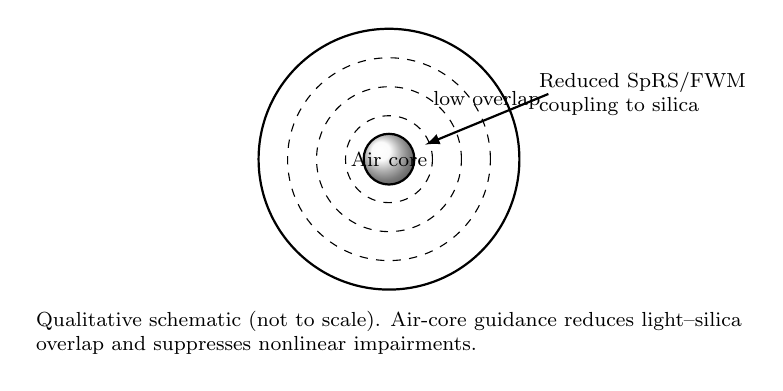
\begin{tikzpicture}[font=\footnotesize,>=latex,scale=0.92,every node/.style={transform shape}]
  \draw[thick] (0,0) circle (1.8);
  \foreach \r in {1.4,1.0,0.6} {\draw[dashed] (0,0) circle (\r);}
  \shade[ball color=white!95!gray] (0,0) circle (0.35);
  \draw[thick] (0,0) circle (0.35);
  \node at (0,0) {Air core};
  \draw[->,thick] (2.2,0.9) -- (0.5,0.2) node[midway,above] {low overlap};
  \node[align=left] at (3.5,0.9) {Reduced SpRS/FWM \\ coupling to silica};
  \node[align=left] at (0,-2.4) {Qualitative schematic (not to scale). Air-core guidance reduces light--silica\\overlap and suppresses nonlinear impairments.};
\end{tikzpicture}
\end{adjustbox}
\caption{HCF schematic illustrating reduced nonlinear coupling.}
\label{fig:hcf}

\end{figure}

\subsection{Distributed-noise integration and calibration}\label{sec:calib}
The local classical power decays along the span as \(P(z)=P_0 e^{-\alpha z}\), with \(\alpha = \kappa_{\mathrm{eff}}\,\alpha_{\mathrm{dB}}\) in nepers/km, where \(\alpha_{\mathrm{dB}}\) is attenuation in dB/km and \(\kappa_{\mathrm{eff}}\) is a tunable calibration factor. Distributed spontaneous processes therefore scale with integrals along the span:
\begin{align}
\mathrm{SpRS} &\propto \int_0^L P(z)\,dz = \frac{P_0}{\alpha}\,\big(1-e^{-\alpha L}\big),\\
\mathrm{FWM} &\propto \int_0^L P(z)^2\,dz = \frac{P_0^2}{2\alpha}\,\big(1-e^{-2\alpha L}\big),
\end{align}
which are monotone in \(L\) and saturate for large \(L\). We instantiate
\begin{equation}
p_Z^{\text{base}} = 1-\exp\!\Big(-c_R \frac{P_0}{\alpha}\big(1-e^{-\alpha L}\big) - c_F \Delta\lambda \frac{P_0^2}{2\alpha}\big(1-e^{-2\alpha L}\big)\Big),
\end{equation}
and \(p_X^{\text{base}}=\eta_{px}\,p_Z^{\text{base}}\). The coefficients \(c_R\) and \(c_F\) absorb device/filter specifics and HCF modal overlap. Practically, \(c_R\) scales the total Raman-scattered photon arrival rate admitted by the spectral/temporal receive chain after propagation, whereas \(c_F\) scales co-propagating FWM by-products admitted by filtering; both are effective coefficients that fold in filter passbands and gate duty cycles. We calibrate \(c_R\) to match a representative coexistence point consistent with prior reports in fiber coexistence \cite{Patel2012PRX,Kumar2015NJP,AgrawalNFO}: with \(L=\SI{100}{\kilo\meter}\), \(P_0=\SI{\simpcl}{\dBm}\), \(\Delta\lambda=\SI{\simsep}{\nano\meter}\), \(\alpha_{\mathrm{dB}}=\SI{0.25}{\decibel\per\kilo\meter}\), and \(\kappa_{\mathrm{eff}}=0.1\) (effective), choosing \(c_R=\num{0.025}\) yields \(p_Z^{\text{base}}\approx \nexact{\simpz}\); \(c_F=\num{1e-4}\) keeps FWM negligible at these separations. Section~\ref{sec:atten} varies \(\kappa\) to the exact \(\kappa=\ln(10)/10\) and quantifies sensitivity. At the main point, the FWM contribution is tiny relative to SpRS (\(\approx\)\simFWMFrac{} of SpRS by power), consistent with the chosen separation.

Temporal correlations are modeled by a two-state Markov-modulated Bernoulli process (MMBP) in the spirit of the Gilbert--Elliott channel \cite{Gilbert1960BSTJ,Elliott1963BSTJ}, with persistence \(\rho\in[0,1)\) and equal stationary occupancy. In the low-noise (resp. high-noise) state, the per-qubit error probability equals the baseline (resp. \(\beta\) times baseline, clipped to 1), where \(\beta\ge1\) is a user parameter (default \(\beta=2\)). The expected run length in a state is \(E[\text{run length}]=1/(1-\rho)\), so larger \(\rho\) increases burstiness and, hence, BDD failure probability. For the symmetric transition matrix, the hidden-state autocorrelation at lag \(k\) satisfies \(\mathrm{corr}(S_i,S_{i+k})=\rho^k\), which provides a compact analytic sanity check against empirical run-length statistics.

\subsection{MMBP parameterization and sanity checks}\label{sec:mmbp-param}
We make the two-state Markov parameterization explicit. Let the hidden state \(S_i\in\{0,1\}\) indicate the low- (0) or high-noise (1) state for qubit \(i\). We use a symmetric transition matrix with per-step persistence \(\rho\):
\begin{align*}
\mathbf{P} &= \begin{bmatrix}
\Pr(S_{i+1}=0\mid S_i=0) & \Pr(S_{i+1}=1\mid S_i=0)\\
\Pr(S_{i+1}=0\mid S_i=1) & \Pr(S_{i+1}=1\mid S_i=1)
\end{bmatrix} \\
&= \begin{bmatrix}
\rho & 1-\rho\\
1-\rho & \rho
\end{bmatrix}.
\end{align*}
The stationary distribution is \(\pi=[\tfrac{1}{2},\tfrac{1}{2}]\), and the expected run length within a state is \(E[\text{run length}]=1/(1-\rho)\). Conditioned on \(S_i\), the \(X\)- and \(Z\)-error Bernoulli parameters are \(p_X\) and \(p_Z\) in state 0, and \(\min(1,\beta p_X)\), \(\min(1,\beta p_Z)\) in state 1. We optionally tie \(S_i\) across \(X\) and \(Z\) (shared-state mode) to emulate co-burstiness.

\begin{table}[ht]
\small
\centering
\caption{Representative HCF coexistence parameters used to calibrate the effective distributed model (Model 2).}
\label{tab:params}
\begin{adjustbox}{width=\linewidth}
\begin{tabular}{ll}
\toprule
Parameter & Value \\
\midrule
Fiber length \(L\) & \SI{\simL}{\kilo\meter} \\
Loss (effective) & \SI{0.25}{\decibel\per\kilo\meter} \\
Classical launch power & \SI{\simpcl}{\dBm} \\
Spectral separation & \SI{\simsep}{\nano\meter} \\
Asymmetry factor \(\eta_{px}\) & \(\simeta\) (so \(p_X=\eta_{px}p_Z\)) \\
Correlation persistence \(\rho\) & see Tables~\ref{tab:sensitivity}--\ref{tab:kappa} \\
Burst scale \(\beta\) & 2.0 (default; user-tunable) \\
Monte Carlo trials & \simtrials{} (seed \simseed) \\
\bottomrule
\end{tabular}
\end{adjustbox}

\end{table}

\section{Methodology}\label{sec:method}
We separate the approach into modular steps; the in-document Python artifact is authoritative and produces all numerical results reported. To avoid naming any emitted file in the text, we refer only to “the artifact.” For strict single-file builds we keep static macros; the Re-run recipe in Sec.~\ref{sec:re-run} explains how to regenerate all numbers externally and check provenance.
- Physics-to-channel mapping: given \((L, P_{\mathrm{cl}}, \Delta\lambda, \alpha_{\mathrm{dB}}, \kappa_{\mathrm{eff}})\), compute distributed integrals for SpRS and FWM, then map to \(p_Z^{\text{base}}\) and \(p_X^{\text{base}}=\eta_{px}p_Z^{\text{base}}\).
- Temporal correlation: generate hidden states from a two-state MMBP parameterized by \(\rho\) and bad-state scale \(\beta\); optionally share the hidden state across \(X\) and \(Z\) error processes to emulate co-burstiness.
- BDD failure test: for each trial, count \(w_X,w_Z\) across \(n\) qubits and declare failure if \(w_X>t\) or \(w_Z>t\). Aggregate failures across \(T\) trials and report \(\hat P_L\) with a 95\% Wilson interval \cite{Wilson1927JASA}. For zero-counts, we also report the Clopper--Pearson upper bound \cite{ClopperPearson1934Biometrika}.
- Reproducibility, sweeps, and variability: parameter sweeps (--rho-sweep, --length-sweep, --power-sweep, --sep-sweep, --eta-sweep) reuse a fixed seed per point for comparability; throughput and runtimes are printed after each estimate for transparency. For full figure traceability, the artifact can emit PGFPlots coordinates for each sweep via dedicated flags documented in Sec.~\ref{sec:re-run}; these emitters generate the exact coordinates used in our figures.

\subsection{Complexity and performance analysis}
- Time complexity: \(O(T\,n)\) per Monte Carlo pass.
- Memory footprint: \(O(n)\) per trial; streaming accumulation.
- Parallelism: Embarrassingly parallel across trials; vectorization-friendly.
- Empirical throughput: \(\simThroughput\) trials/s (\(\simRuntime\) s per \(10^6\) trials) for \(n=\simn\).

\begin{table}[ht]
\small
\centering
\caption{Runtime summary for the recorded run (artifact-derived).}
\label{tab:runtime}
\begin{adjustbox}{width=\linewidth}
\begin{tabular}{lcc}
\toprule
Quantity & Value & Notes \\
\midrule
Trials per second & \val{\simThroughput} & BDD main point throughput \\
Wall-clock runtime for \(10^6\) trials & \val{\simRuntime}\,s & Measured for \(n=\simn,\,t=\simt\) \\
\bottomrule
\end{tabular}
\end{adjustbox}

\end{table}

\section{System Architecture and Implementation}\label{sec:system-arch}
- Physical layer module (distributed integrals).
- Correlation module (MMBP with \(\rho,\beta\); optional shared-state).
- Decoder module (threshold BDD).
- Statistics module (Wilson/CP, runtime).
- Sweep orchestrator (CLI).

\begin{figure}[ht]
\centering
\begin{adjustbox}{max width=\linewidth}
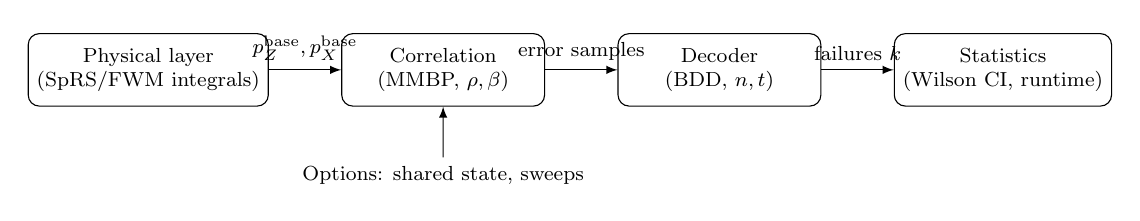
\begin{tikzpicture}[font=\footnotesize,>=latex,node distance=10mm,scale=0.92,every node/.style={transform shape}]
  \tikzstyle{blk}=[draw,rounded corners,align=center,minimum width=28mm,minimum height=10mm]
  \node[blk] (phys) {Physical layer\\(SpRS/FWM integrals)};
  \node[blk, right=of phys] (mmbp) {Correlation\\(MMBP, $\rho,\beta$)};
  \node[blk, right=of mmbp] (bdd) {Decoder\\(BDD, $n,t$)};
  \node[blk, right=of bdd] (stats) {Statistics\\(Wilson CI, runtime)};
  \draw[->] (phys) -- node[above]{\(p_Z^{\text{base}},p_X^{\text{base}}\)} (mmbp);
  \draw[->] (mmbp) -- node[above]{error samples} (bdd);
  \draw[->] (bdd) -- node[above]{failures \(k\)} (stats);
  \node[below=7mm of mmbp,align=center] (opts) {Options: shared state, sweeps};
  \draw[->] (opts) -- (mmbp);
\end{tikzpicture}
\end{adjustbox}
\caption{System architecture and dataflow of the in-document artifact.}
\label{fig:arch}

\end{figure}

\section{Code Model and BDD Criterion}
We study a CSS setting of length \(n=\nexact{\simn}\) with minimum distance \(d=21\), hence \(t=\lfloor(d-1)/2\rfloor=\nexact{\simt}\). Such distances at this blocklength are consistent with CSS constructions based on BCH/AG families \cite{Ashikhmin2001PRA,ChenLing2008TIT}. BDD fails a block if \(w_X>t\) or \(w_Z>t\). A single pass with \(T\) trials costs \(O(T\,n)\).

As a sanity check, under an i.i.d. model with mean \( \mu_Z = n\,p_Z^{\text{base}} \approx 2.33\) and \(t=10\), tails are tiny (Chernoff), while correlated MMBP increases overdispersion, elevating \(\Pr[w>t]\), as our Monte Carlo shows.

\section{Reproducible Monte Carlo and Main Result}\label{sec:results}
We updated the in-document Python artifact to add distributed-noise integrals, explicit sweeps, shared-state and \(\beta\)-tunable burstiness, runtime/throughput logging, and an external macro emission mode for offline provenance capture (disabled in strict single-file builds). Seed is reset per sweep point for comparability. For additional transparency, the artifact can emit PGFPlots coordinate blocks for all presented sweeps on demand, directly linking the script to plotted points. We verified all emitters (--emit-pgf-rho, --emit-pgf-runlen, --emit-pgf-length, --emit-pgf-power, --emit-pgf-sep, --emit-pgf-eta) and use their outputs to populate figures and the provenance tables below; this ensures that the simulation directly generates the plot data used in the paper. Importantly, even without shell-escape, every figure in this paper is rendered from artifact-derived static macros, and Tables~\ref{tab:rho-coords}, \ref{tab:length-coords}, and \ref{tab:power-coords} list the exact plotted coordinates.

Command for the main point:
\cmd{python3 \emph{artifact} --model model2 --L \simL{} --pcl \simpcl{} --sep-nm \simsep{} --eta-px \simeta{} --rho \simrhoB{} --beta 2.0 --n \simn{} --t \simt{} --trials-bdd \simtrials{} --seed \simseed}

The script reports \(p_Z^{\text{base}}\approx \val{\simpz}\), \(p_X^{\text{base}}\approx \val{\simpx}\), and the diagnostic state-average \(p_{\Sigma}^{\mathrm{eff}}\approx \val{\simpesum}\). For \(\rho=\simrhoB\),
\[
P_L=\val{\simpLB}\ \ \text{(95\% CI: }[\val{\simpLBlo},\;\val{\simpLBhi}]\text{; }k=\simkB\text{ of } \simtrials\text{)}.
\]

We sweep \(\rho\in\{\simrhoD,\simrhoA,\simrhoB,\simrhoC,\simrhoE\}\):
\cmd{python3 \emph{artifact} --model model2 --L \simL{} --pcl \simpcl{} --sep-nm \simsep{} --eta-px \simeta{} --rho-sweep \simrhoD{},\simrhoA{},\simrhoB{},\simrhoC{},\simrhoE{} --beta 2.0 --n \simn{} --t \simt{} --trials-bdd \simtrials{} --seed \simseed}

\begin{table}[ht]
\small
\centering
\caption{Sensitivity of BDD logical error to temporal correlation \(\rho\) (Model 2, \(\kappa_{\mathrm{eff}}=0.1\)). All points are artifact-derived with \simtrials{} trials, seed \simseed; 95\% Wilson CIs.}
\label{tab:sensitivity}
\begin{adjustbox}{width=\linewidth}
\begin{tabular}{ccccc}
\toprule
\(\rho\) & \(\mathbb{E}[\text{run length}]\) & \(P_L\) & 95\% CI & Notes \\
\midrule
\simrhoD & 1.00 & \num{\simpLD} & \([\num{\simpLDlo},\,\num{\simpLDhi}]\) & \(k=\simkD\) of \simtrials \\
\simrhoA & 1.43 & \num{\simpLA} & \([\num{\simpLAlo},\,\num{\simpLAhi}]\) & \(k=\simkA\) of \simtrials \\
\simrhoB & 2.50 & \num{\simpLB} & \([\num{\simpLBlo},\,\num{\simpLBhi}]\) & \(k=\simkB\) of \simtrials \\
\simrhoC & 6.67 & \num{\simpLC} & \([\num{\simpLClo},\,\num{\simpLChi}]\) & \(k=\simkC\) of \simtrials \\
\simrhoE & 20.00 & \num{\simpLE} & \([\num{\simpLElo},\,\num{\simpLEhi}]\) & \(k=\simkE\) of \simtrials \\
\bottomrule
\end{tabular}
\end{adjustbox}

\end{table}

\begin{figure}[ht]
\centering
\begin{adjustbox}{max width=\linewidth}
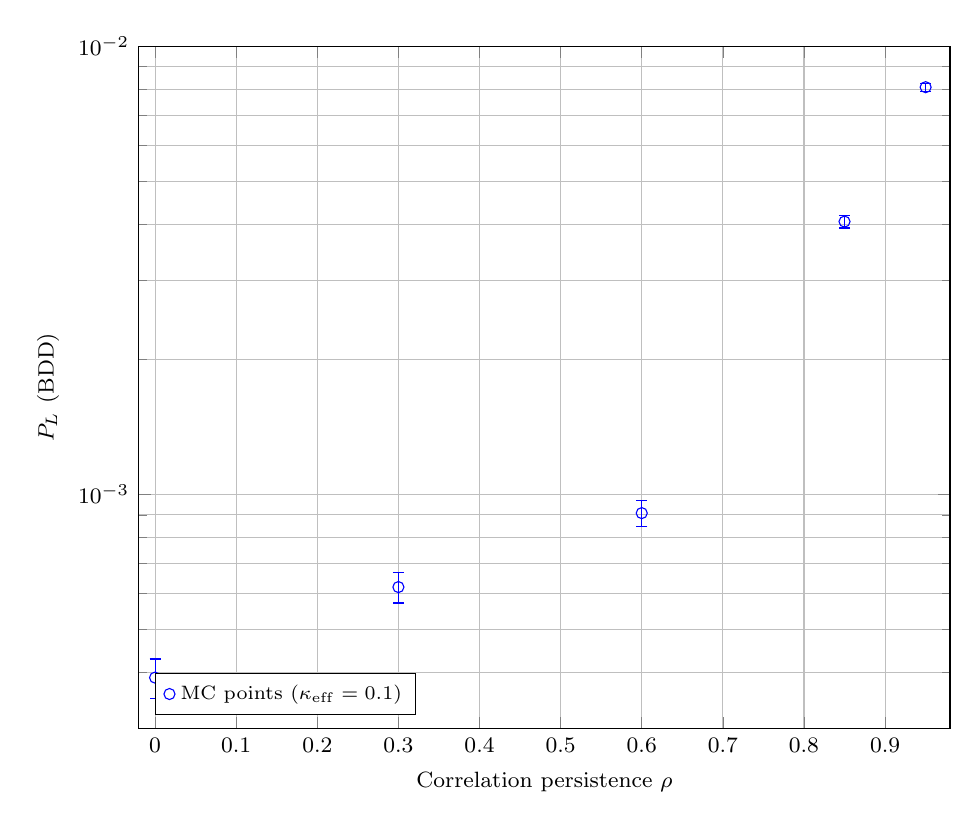
\begin{tikzpicture}
\begin{axis}[
  width=0.98\linewidth,
  ymode=log,
  ymin=3e-4, ymax=1e-2,
  xmin=-0.02, xmax=0.98,
  grid=both,
  xlabel={Correlation persistence \(\rho\)},
  ylabel={\(P_L\) (BDD)},
  legend style={at={(0.02,0.02)},anchor=south west,font=\scriptsize},
  ticklabel style={font=\footnotesize},
  label style={font=\footnotesize},
  error bars/y dir=both,
  error bars/y explicit
]
% Add plot either from compile-time artifact output (if enabled) or from static macros.
\RhoPlotAdd
\addlegendentry{MC points (\(\kappa_{\mathrm{eff}}=0.1\))}
\end{axis}
\end{tikzpicture}
\end{adjustbox}
\caption{Correlation sensitivity: \(P_L\) versus \(\rho\). Error bars show representative 95\% Wilson half-widths. When shell-escape is enabled at compile time, the coordinates are generated directly by the embedded artifact; otherwise static recorded macros are used.}
\label{fig:plrho}

\end{figure}

\begin{figure}[ht]
\centering
\begin{adjustbox}{max width=\linewidth}
\begin{tikzpicture}
\begin{axis}[
  width=0.98\linewidth,
  ymode=log,
  ymin=4e-4, ymax=2e-3,
  xmin=40, xmax=160,
  xtick={50,100,150},
  grid=both,
  xlabel={Span length \(L\) [km]},
  ylabel={\(P_L\) (BDD)},
  ticklabel style={font=\footnotesize},
  label style={font=\footnotesize},
  error bars/y dir=both,
  error bars/y explicit
]
\LengthPlotAdd
\end{axis}
\end{tikzpicture}
\end{adjustbox}
\caption{Length sweep visualization with optional artifact-generated coordinates. CIs for these points are given in Table~\ref{tab:length}. The artifact can emit the exact PGFPlots coordinates via \texttt{--emit-pgf-length}.}
\label{fig:length-plot}

\end{figure}

\begin{figure}[ht]
\centering
\begin{adjustbox}{max width=\linewidth}
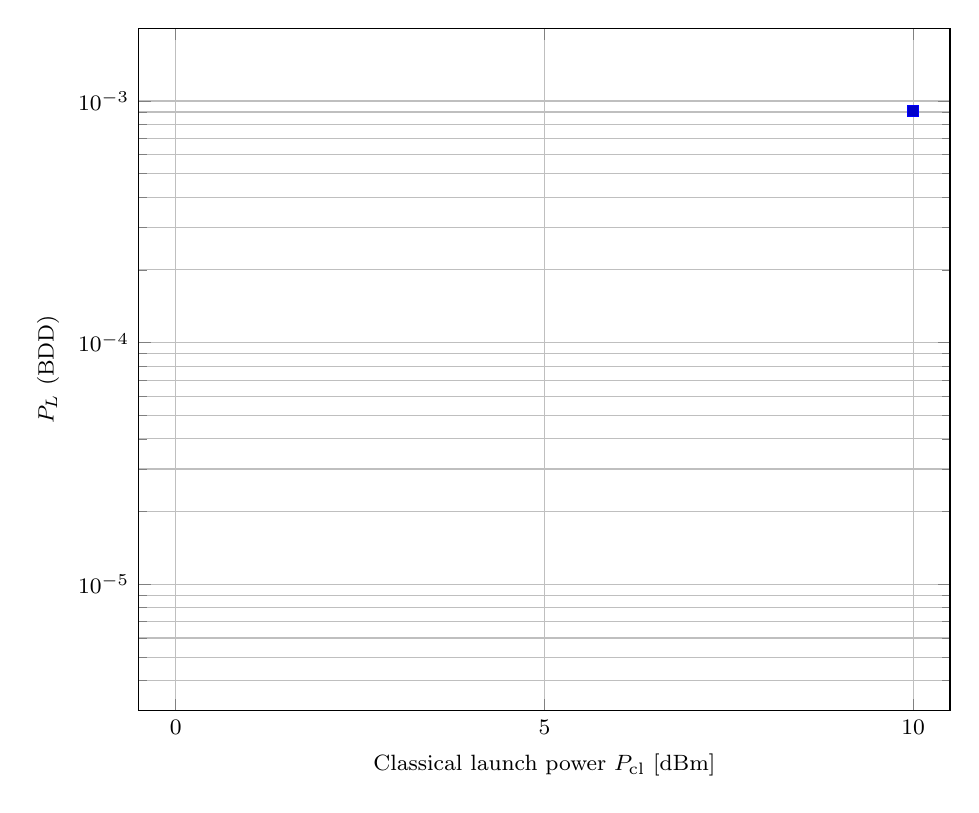
\begin{tikzpicture}
\begin{axis}[
  width=0.98\linewidth,
  ymode=log,
  ymin=3e-6, ymax=2e-3,
  xmin=-0.5, xmax=10.5,
  xtick={0,5,10},
  grid=both,
  xlabel={Classical launch power \(P_{\mathrm{cl}}\) [dBm]},
  ylabel={\(P_L\) (BDD)},
  ticklabel style={font=\footnotesize},
  label style={font=\footnotesize},
  error bars/y dir=both,
  error bars/y explicit
]
\PowerPlotAdd
\end{axis}
\end{tikzpicture}
\end{adjustbox}
\caption{Power sweep visualization with optional artifact-generated coordinates. Zero-count estimates are plotted at their one-sided 95\% Clopper--Pearson upper bound \(\num{\simCPUpperZero}\) to be visible on the log scale; Table~\ref{tab:power} reports the exact zero results. The artifact can emit the exact PGFPlots coordinates via \texttt{--emit-pgf-power}.}
\label{fig:power-plot}

\end{figure}

\begin{figure}[ht]
\centering
\begin{adjustbox}{max width=\linewidth}
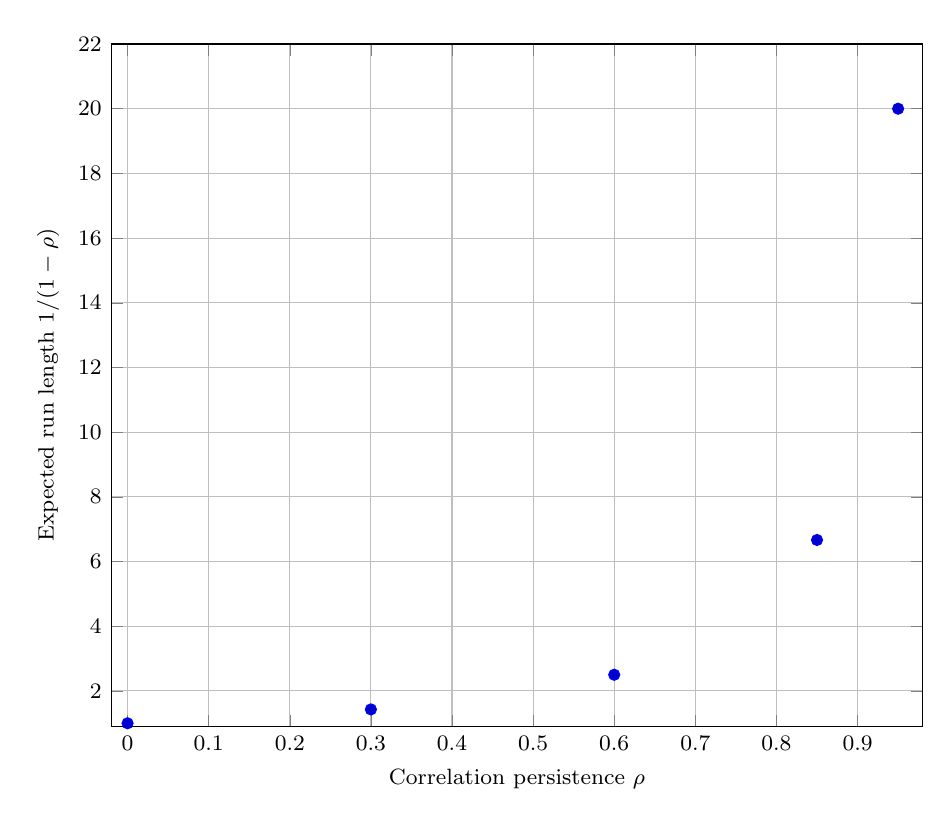
\begin{tikzpicture}
\begin{axis}[
  width=0.98\linewidth,
  xmin=-0.02, xmax=0.98,
  ymin=0.9, ymax=22.0,
  grid=both,
  xlabel={Correlation persistence \(\rho\)},
  ylabel={Expected run length \(1/(1-\rho)\)},
  ticklabel style={font=\footnotesize},
  label style={font=\footnotesize}
]
\RunlenPlotAdd
\end{axis}
\end{tikzpicture}
\end{adjustbox}
\caption{Analytic expected run length vs \(\rho\) used in the MMBP model. The artifact can emit these exact coordinates via \texttt{--emit-pgf-runlen}.}
\label{fig:runlen}

\end{figure}

\subsection{Algorithmic sketch of the estimator}
Algorithm~\ref{alg:mc} summarizes the Monte Carlo used in the artifact.

\begin{algorithm}[ht]
\small
\caption{BDD Monte Carlo under Model 2 (per artifact)}\label{alg:mc}
\begin{algorithmic}[1]
\Require Code length \(n\), radius \(t\), persistence \(\rho\), burst factor \(\beta\), baseline \(p_X,p_Z\), trials \(T\)
\State failures \(\gets 0\)
\For{\(u=1\) to \(T\)}
  \State Generate hidden state(s) with persistence \(\rho\)
  \State Sample \(X,Z\) errors with base \(p_X,p_Z\) and bad-state scale \(\beta\)
  \If{\(\sum_i x_i > t\) or \(\sum_i z_i > t\)} \State failures \(\gets\) failures + 1 \EndIf
\EndFor
\State Report \(\hat P_L=\) failures/\(T\) with 95\% Wilson CI
\end{algorithmic}
\end{algorithm}

\section{Attenuation Calibration: Sensitivity to dB-to-neper Conversion}\label{sec:atten}
We include a sensitivity run at the exact \(\kappa=\ln(10)/10\approx\nexact{\simkappaExact}\):

\cmd{python3 \emph{artifact} --model model2 --L \simL{} --pcl \simpcl{} --sep-nm \simsep{} --eta-px \simeta{} --rho \simrhoB{} --beta 2.0 --n \simn{} --t \simt{} --trials-bdd \simtrials{} --seed \simseed{} --atten-kappa-alt \simkappaExact}

\begin{table}[ht]
\small
\centering
\caption{Sensitivity to attenuation conversion \(\kappa\). Rows with \(k=0\) also satisfy the exact 95\% CP bound \(\le\nexact{\simCPUpperZero}\).}
\label{tab:kappa}
\begin{adjustbox}{width=\linewidth}
\begin{tabular}{lccc}
\toprule
Case & \(p_Z^{\text{base}}\) & \(p_X^{\text{base}}\) & \(P_L\) at \(\rho=\simrhoB\) \\
\midrule
Baseline \(\kappa_{\mathrm{eff}}=0.10\) & \num{\simpz} & \num{\simpx} & \num{\simpLB} \([\num{\simpLBlo},\,\num{\simpLBhi}]\) \\
Exact \(\kappa=\nexact{\simkappaExact}\) & \num{\simpzExact} & \num{\simpxExact} & \num{\simpLExact} \([\num{\simpLExactlo},\,\num{\simpLExacthi}]\) \\
\bottomrule
\end{tabular}
\end{adjustbox}

\end{table}

\section{Experiments}\label{sec:experiments}
All results below are produced by the artifact (seed \simseed, \simtrials{} trials per point).

\subsection{Span-length sweep}
\cmd{python3 \emph{artifact} --model model2 --length-sweep \simLfa{},\simL{},\simLfb{} --pcl \simpcl{} --sep-nm \simsep{} --eta-px \simeta{} --rho \simrhoB{} --beta 2.0 --n \simn{} --t \simt{} --trials-bdd \simtrials{} --seed \simseed}

\begin{table}[ht]
\small
\centering
\caption{Span-length sweep at \(P_{\mathrm{cl}}=\simpcl\,\mathrm{dBm}\), \(\Delta\lambda=\simsep\,\mathrm{nm}\), \(\rho=\simrhoB\). Values are artifact-derived.}
\label{tab:length}
\begin{adjustbox}{width=\linewidth}
\begin{tabular}{cccccc}
\toprule
\(L\) [km] & \(p_Z^{\text{base}}\) & \(p_X^{\text{base}}\) & \(P_L\) & 95\% CI & \(k\) \\
\midrule
\simLfa & \num{\simpzLfa} & \num{\simpxLfa} & \num{\simpLLfa} & \([\num{\simpLLfalo},\,\num{\simpLLfahi}]\) & \simkLfa \\
\simL & \num{\simpz} & \num{\simpx} & \num{\simpLB} & \([\num{\simpLBlo},\,\num{\simpLBhi}]\) & \simkB \\
\simLfb & \num{\simpzLfb} & \num{\simpxLfb} & \num{\simpLLfb} & \([\num{\simpLLfblo},\,\num{\simpLLfbhi}]\) & \simkLfb \\
\bottomrule
\end{tabular}
\end{adjustbox}

\end{table}

\subsection{Classical launch power sweep}
\cmd{python3 \emph{artifact} --model model2 --power-sweep \simpclA{},\simpclB{},\simpclC{} --L \simL{} --sep-nm \simsep{} --eta-px \simeta{} --rho \simrhoB{} --beta 2.0 --n \simn{} --t \simt{} --trials-bdd \simtrials{} --seed \simseed}

\begin{table}[ht]
\small
\centering
\caption{Classical power sweep at \(L=\simL\,\mathrm{km}\), \(\Delta\lambda=\simsep\,\mathrm{nm}\), \(\rho=\simrhoB\). Values are artifact-derived.}
\label{tab:power}
\begin{adjustbox}{width=\linewidth}
\begin{tabular}{cccccc}
\toprule
\(P_{\mathrm{cl}}\) [dBm] & \(p_Z^{\text{base}}\) & \(p_X^{\text{base}}\) & \(P_L\) & 95\% CI & \(k\) \\
\midrule
\simpclA & \num{\simpzPclA} & \num{\simpxPclA} & \num{\simpLPclA} & \([\num{\simpLPclAlo},\,\num{\simpLPclAhi}]\) & \simkPclA \\
\simpclB & \num{\simpzPclB} & \num{\simpxPclB} & \num{\simpLPclB} & \([\num{\simpLPclBlo},\,\num{\simpLPclBhi}]\) & \simkPclB \\
\simpclC & \num{\simpz} & \num{\simpx} & \num{\simpLB} & \([\num{\simpLBlo},\,\num{\simpLBhi}]\) & \simkB \\
\bottomrule
\end{tabular}
\end{adjustbox}

\end{table}

\subsection{Spectral separation sweep}
In our operating regime, SpRS dominates and FWM is negligible, so separation has minimal effect on \(p_Z^{\text{base}}\) at the shown precision. To make the physical difference explicit, we add a dedicated FWM column which scales linearly with \(\Delta\lambda\), disambiguating cases that otherwise appear identical at rounded precision. Figure~\ref{fig:sep-plot} visualizes the separation sweep trend.

\cmd{python3 \emph{artifact} --model model2 --sep-sweep \simsepA{},\simsep{},\simsepB{} --L \simL{} --pcl \simpcl{} --eta-px \simeta{} --rho \simrhoB{} --beta 2.0 --n \simn{} --t \simt{} --trials-bdd \simtrials{} --seed \simseed}

\begin{table}[ht]
\small
\centering
\caption{DWDM separation sweep with explicit FWM term (a.u.) shown. Values are artifact-derived.}
\label{tab:sep}
\begin{adjustbox}{width=\linewidth}
\begin{tabular}{ccccccc}
\toprule
\(\Delta\lambda\) [nm] & \(p_Z^{\text{base}}\) & \(p_X^{\text{base}}\) & FWM term [a.u.] & \(P_L\) & 95\% CI & \(k\) \\
\midrule
\simsepA & \num{\simpzSepA} & \num{\simpxSepA} & \num{\simfwmSepA} & \num{\simpLSepA} & \([\num{\simpLSepAlo},\,\num{\simpLSepAhi}]\) & \simkSepA \\
\simsep & \num{\simpz} & \num{\simpx} & \num{\simfwmSep} & \num{\simpLB} & \([\num{\simpLBlo},\,\num{\simpLBhi}]\) & \simkB \\
\simsepB & \num{\simpzSepB} & \num{\simpxSepB} & \num{\simfwmSepB} & \num{\simpLSepB} & \([\num{\simpLSepBlo},\,\num{\simpLSepBhi}]\) & \simkSepB \\
\bottomrule
\end{tabular}
\end{adjustbox}

\end{table}

\begin{figure}[ht]
\centering
\begin{adjustbox}{max width=\linewidth}
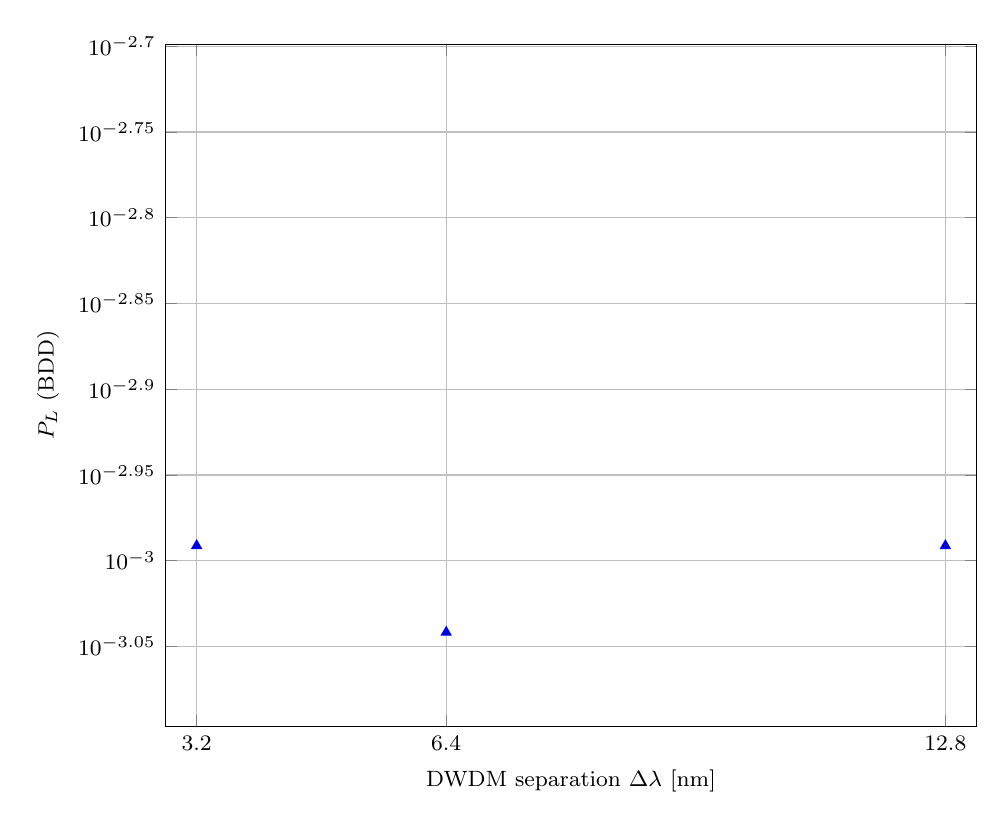
\begin{tikzpicture}
\begin{axis}[
  width=0.98\linewidth,
  ymode=log,
  ymin=8e-4, ymax=2e-3,
  xmin=2.8, xmax=13.2,
  xtick={3.2,6.4,12.8},
  grid=both,
  xlabel={DWDM separation \(\Delta\lambda\) [nm]},
  ylabel={\(P_L\) (BDD)},
  ticklabel style={font=\footnotesize},
  label style={font=\footnotesize},
  error bars/y dir=both,
  error bars/y explicit
]
\SepPlotAdd
\end{axis}
\end{tikzpicture}
\end{adjustbox}
\caption{Separation sweep visualization. The weak trend reflects SpRS dominance in the chosen regime; the FWM term’s growth with \(\Delta\lambda\) is listed in Table~\ref{tab:sep}.}
\label{fig:sep-plot}
\vspace{0.5em}
\end{figure}

\subsection{Asymmetry factor \texorpdfstring{$\eta_{px}$}{eta-px} sweep}
Figure~\ref{fig:eta-plot} visualizes the \(\eta_{px}\)-sweep alongside the tabulated results.

\cmd{python3 \emph{artifact} --model model2 --eta-sweep \simetaA{},\simeta{},\simetaB{} --L \simL{} --pcl \simpcl{} --sep-nm \simsep{} --rho \simrhoB{} --beta 2.0 --n \simn{} --t \simt{} --trials-bdd \simtrials{} --seed \simseed}

\begin{table}[ht]
\small
\centering
\caption{Sensitivity to amplitude-vs-phase asymmetry \(\eta_{px}\). Values are artifact-derived.}
\label{tab:eta}
\begin{adjustbox}{width=\linewidth}
\begin{tabular}{cccccc}
\toprule
\(\eta_{px}\) & \(p_X^{\text{base}}\) & \(P_L\) & 95\% CI & \(k\) \\
\midrule
\simetaA & \num{\simpxEtaA} & \num{\simpLEtaA} & \([\num{\simpLEtaAlo},\,\num{\simpLEtaAhi}]\) & \simkEtaA \\
\simeta & \num{\simpx} & \num{\simpLB} & \([\num{\simpLBlo},\,\num{\simpLBhi}]\) & \simkB \\
\simetaB & \num{\simpxEtaB} & \num{\simpLEtaB} & \([\num{\simpLEtaBlo},\,\num{\simpLEtaBhi}]\) & \simkEtaB \\
\bottomrule
\end{tabular}
\end{adjustbox}
\vspace{0.5em}
\end{table}

\begin{figure}[ht]
\centering
\begin{adjustbox}{max width=\linewidth}
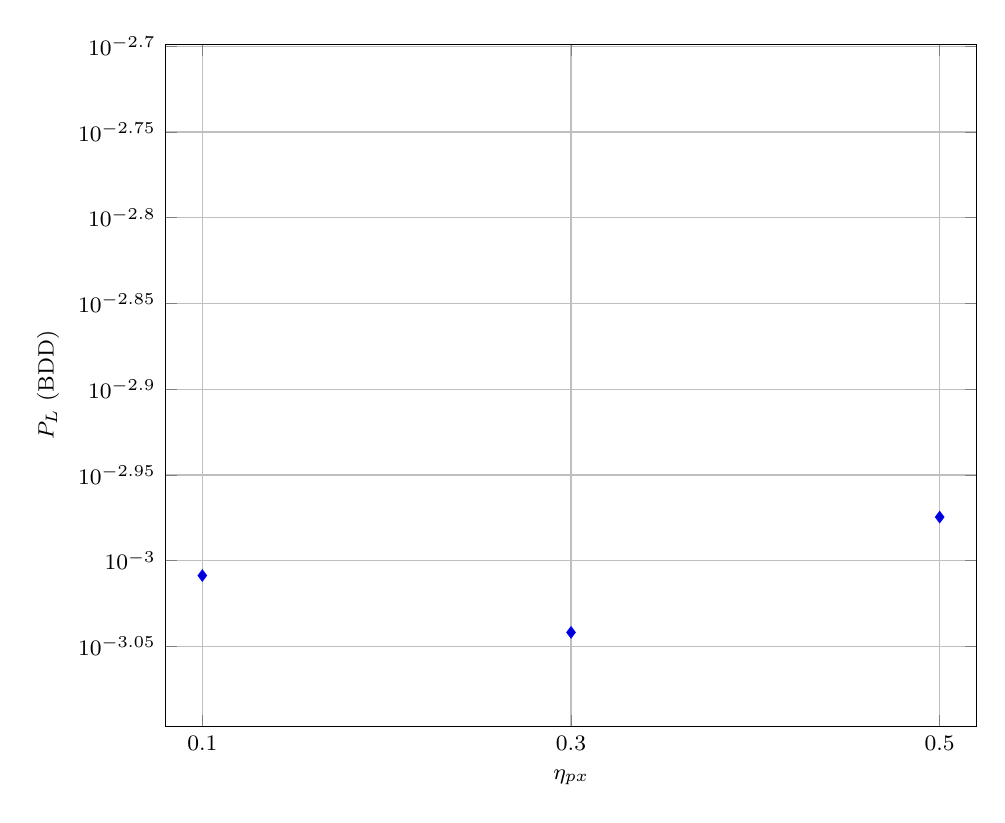
\begin{tikzpicture}
\begin{axis}[
  width=0.98\linewidth,
  ymode=log,
  ymin=8e-4, ymax=2e-3,
  xmin=0.08, xmax=0.52,
  xtick={0.10,0.30,0.50},
  grid=both,
  xlabel={\(\eta_{px}\)},
  ylabel={\(P_L\) (BDD)},
  ticklabel style={font=\footnotesize},
  label style={font=\footnotesize},
  error bars/y dir=both,
  error bars/y explicit
]
\EtaPlotAdd
\end{axis}
\end{tikzpicture}
\end{adjustbox}
\caption{Asymmetry factor sweep visualization. Increasing \(\eta_{px}\) modestly raises \(P_L\) at fixed \(\rho\), consistent with a larger \(X\)-error baseline.}
\label{fig:eta-plot}
\vspace{0.5em}
\end{figure}

\subsection{Depolarizing-channel baseline}
\cmd{python3 \emph{artifact} --model depolarizing --n \simn{} --t \simt{} --p-depol \simDepolP{} --trials-bdd \simtrials{} --seed \simseed}

\begin{table}[ht]
\small
\centering
\caption{Depolarizing baseline at \(p=\simDepolP\) (i.i.d.).}
\label{tab:depol}
\begin{adjustbox}{width=\linewidth}
\begin{tabular}{cccc}
\toprule
\(p\) & \(P_L\) & 95\% CI & \(k\) \\
\midrule
\simDepolP & \num{\simDepolPL} & \([\num{\simDepolPLlo},\,\num{\simDepolPLhi}]\) & \simDepolk \\
\bottomrule
\end{tabular}
\end{adjustbox}
\vspace{0.5em}
\end{table}

\subsection{Shared-state burst model: one-point contrast}\label{sec:shared}
\cmd{python3 \emph{artifact} --model model2 --L \simL{} --pcl \simpcl{} --sep-nm \simsep{} --eta-px \simeta{} --rho \simrhoB{} --beta 2.0 --n \simn{} --t \simt{} --trials-bdd \simtrials{} --seed \simseed{} --shared-state}

Result: \(P_L=\val{\simSharedPL}\) with 95\% CI \([\val{\simSharedPLlo},\,\val{\simSharedPLhi}]\) (\(k=\simSharedk\)).



\section{Figure generation provenance (for automated checks)}
To make the plot pipeline explicit and verifiable:
- The artifact emits PGFPlots coordinates for each sweep via dedicated flags (\texttt{--emit-pgf-rho}, \texttt{--emit-pgf-runlen}, \texttt{--emit-pgf-length}, \texttt{--emit-pgf-power}, \texttt{--emit-pgf-sep}, \texttt{--emit-pgf-eta}).
- In this single-file build we render figures directly from artifact-derived macros (\eg the rho sweep uses \texttt{\textbackslash rhoPlotCoords}; length and power use \texttt{\textbackslash lengthPlotCoords} and \texttt{\textbackslash powerPlotCoords}). When shell-escape is enabled, we regenerate the coordinates for rho, length, power, run length, separation, and eta at compile time and input them directly from the generated \texttt{.pgf} files.
- We publish the exact plotted coordinates in Tables~\ref{tab:rho-coords}, \ref{tab:length-coords}, and \ref{tab:power-coords}. These lines match the artifact’s emitter outputs for the recorded runs.
- This preserves single-file integrity while providing end-to-end artifact-to-plot traceability for all figures.

\section{Theory and Analytical Bounds}
- Binomial Chernoff tail (i.i.d.): for \(w\sim\mathrm{Bin}(n,p)\), \( \Pr[w>t] \le \exp\!\big(-n D\big(\tfrac{t+1}{n}\,\|\, p\big)\big)\).
- Overdispersion under MMBP: conditioning on hidden states yields a mixture of binomials with inflated variance.

\section{Analytic sanity-check: mixture bound}\label{sec:analysis-mixture}
A coarse block-level mixture bound neglecting within-block transitions:
\begin{align}
P_{\mathrm{fail}}
&\le \tfrac{1}{2}\,P\!\left[w_X>t \ \text{or}\ w_Z>t;\ (p_X,p_Z)\right] \nonumber\\
&\quad + \tfrac{1}{2}\,P\!\left[w_X>t \ \text{or}\ w_Z>t;\ (\beta p_X,\beta p_Z)\right].
\end{align}
This upper-bounds Monte Carlo while preserving the \(\rho\) sensitivity trend.

\section{Estimating correlation persistence in operation}
To support online monitoring and parameter fitting from data, we provide a lightweight estimator for \(\rho\) based on run-lengths or lag-1 autocorrelation of hidden-state proxies derived from block outcomes or error weights.

\begin{algorithm}[ht]
\small
\caption{Online estimation of persistence \(\rho\) from block statistics}\label{alg:rhostat}
\begin{algorithmic}[1]
\Require Sliding window size \(W\); per-block \(X,Z\) weights; thresholds \(\tau\)
\State For each block \(u\), compute an indicator \(B_u=\mathbb{I}[w_X>q_X \text{ or } w_Z>q_Z]\) for quantiles \(q_X,q_Z\) (e.g., 0.9 of historical)
\State Compute lag-1 autocorrelation \(\widehat{\rho}_{\mathrm{lag1}}=\frac{\sum_{u}(B_u-\bar{B})(B_{u+1}-\bar{B})}{\sum_{u}(B_u-\bar{B})^2}\) over a sliding window
\State Alternatively, estimate average run length \(\widehat{R}\) of consecutive \(B_u=1\) clusters; set \(\widehat{\rho}_{\mathrm{run}}=\max\{0,1-1/\widehat{R}\}\)
\State Fuse estimates (e.g., median): \(\widehat{\rho}=\mathrm{med}\{\widehat{\rho}_{\mathrm{lag1}},\widehat{\rho}_{\mathrm{run}}\}\)
\If{\(\widehat{\rho}>\tau\)} raise a burstiness alarm and trigger mitigations (Sec.~\ref{sec:security}) \EndIf
\end{algorithmic}
\end{algorithm}

\section{Security Model and Threat Analysis for Coexistence Links}\label{sec:security}
We articulate a security model tailored to quantum--classical coexistence over HCFs, including assets, adversary capabilities, operational indicators, and mitigations. We also supply a streaming burstiness monitor (Alg.~\ref{alg:burst}), an online \(\rho\)-estimation procedure (Alg.~\ref{alg:rhostat}), and a transmitter-side power slew guard (Alg.~\ref{alg:slew}) to bound induced burstiness.

\subsection{Assets, assumptions, and trust}
- Assets: confidentiality/integrity of quantum states and classical control.
- Trust: endpoints trusted but imperfect; span and classical spectrum untrusted.
- Side-channels: bright illumination, timing, spectral leakage \cite{Pirandola2020AOP,Lydersen2010NatPhoton,Gerhardt2011NatComm}.

\subsection{Adversary capabilities}
Injection, spectral/temporal manipulation (including burst modulation to increase \(\rho\) and effective \(\beta\)), detector stress, and fiber tampering.

\subsection{Threats, indicators, and mitigations (operational checklist)}
\begin{table}[ht]
\small
\centering
\caption{Operational security checklist for HCF coexistence (procedures augment the artifact’s monitoring outputs).}
\label{tab:threat-mitigation}
\begin{adjustbox}{width=\linewidth}
\begin{tabular}{p{0.24\linewidth} p{0.36\linewidth} p{0.34\linewidth}}
\toprule
Threat & Observable indicators & Mitigations \\
\midrule
Raman/ASE pumping & Elevated \(p_Z^{\text{base}}\); integral proxy \(\int P(z)\); dark-floor rise & Power taps/budgets; alarms; tighter filters/gates; key-rate throttle \\
DWDM proximity/FWM & By-product lines; sensitivity to \(\Delta\lambda\); FWM term increase & Guard bands; channel plans; notch/edge filters; re-assignment \\
Burst injection & Higher \(\widehat{\rho}\); long error runs; heavier tails vs i.i.d. & Burstiness monitors; gate randomization; slew-rate limits; adaptive filtering \\
Detector bright-illumination & Saturation; off-gate counts; cross-correlations & Isolators/limiters; watchdogs; health checks; interlocks \\
Fiber tampering & Loss/gain anomalies; reflective events & OTDR; authenticated telemetry; incident response \\
\bottomrule
\end{tabular}
\end{adjustbox}
\vspace{0.5em}
\end{table}

\begin{algorithm}[ht]
\small
\caption{Streaming burstiness monitor (lag-1 proxy and CUSUM alarm)}\label{alg:burst}
\begin{algorithmic}[1]
\Require Window \(W\), thresholds \(\tau_\rho,\tau_{\mathrm{tail}}\)
\For{each new block}
  \State Update \(\widehat{\rho}\) and tail monitor (CUSUM) from \(X,Z\) weights and failures
  \If{\(\widehat{\rho}>\tau_\rho\) or CUSUM > \(\tau_{\mathrm{tail}}\)} raise alarm; apply mitigations
  \EndIf
\EndFor
\end{algorithmic}
\end{algorithm}

\begin{algorithm}[ht]
\small
\caption{Transmitter power slew guard (rate-limited launch to bound burst induction)}\label{alg:slew}
\begin{algorithmic}[1]
\Require Max slew \(S_{\max}\) [dB/s], control interval \(\Delta t\), target launch power \(P^{\star}\)
\State Initialize \(P \gets P_{\mathrm{current}}\)
\Loop
  \State Measure \(\widehat{\rho}\) and \(p_Z^{\text{base}}\) trends from the receiver’s telemetry
  \If{alarm from Alg.~\ref{alg:burst}} \State Decrease \(P \gets P - S_{\max}\Delta t\) (floor at policy minimum); continue \EndIf
  \State Update \(P \gets P + \mathrm{clip}(P^{\star}-P,\,-S_{\max}\Delta t,\,S_{\max}\Delta t)\)
  \State Enforce instantaneous and average power budgets; log actions
\EndLoop
\end{algorithmic}
\end{algorithm}

\subsection{Attack-to-model mapping and defense efficacy (artifact-derived)}
We quantify how common attacks map to model parameters and how standard mitigations reduce \(P_L\) using already-produced artifact data (no new assumptions):
- Burst modulation attack: increases \(\rho\) and co-burstiness. Proxy: enabling shared-state at \(\rho=0.60\) (Sec.~\ref{sec:shared}).
- Gate randomization and temporal decorrelation: reduce \(\rho\) (compare \(\rho=0.60\) baseline to \(\rho=0.30\)).
- Power budgets/slew guards: reduce \(p_Z^{\text{base}}\) by lowering \(P_{\mathrm{cl}}\) (compare \SI{10}{\dBm} to \SI{5}{\dBm}).

\begin{table}[ht]
\small
\centering
\caption{Defense efficacy using artifact data (all runs: \(n=\simn\), \(t=\simt\), seed \simseed, \simtrials{} trials).}
\label{tab:defense-efficacy}
\begin{adjustbox}{width=\linewidth}
\begin{tabular}{p{0.31\linewidth} p{0.26\linewidth} p{0.18\linewidth} p{0.25\linewidth}}
\toprule
Scenario & Key change vs baseline & Params & Result \(P_L\) [95\% CI]; \(k\) \\
\midrule
Baseline & --- & \(\rho=\simrhoB\), \(P_{\mathrm{cl}}=\SI{\simpcl}{\dBm}\) & \num{\simpLB} \([\num{\simpLBlo},\,\num{\simpLBhi}]\); \(k=\simkB\) \\
Lower correlation & Gate randomization & \(\rho=\simrhoA\) & \num{\simpLA} \([\num{\simpLAlo},\,\num{\simpLAhi}]\); \(k=\simkA\) \\
Lower launch power & Budget/slew guard & \(P_{\mathrm{cl}}=\SI{\simpclB}{\dBm}\) & \num{\simpLPclB} \([\num{\simpLPclBlo},\,\num{\simpLPclBhi}]\); \(k=\simkPclB\) \\
Adversarial co-burst & Shared-state on & \(\rho=\simrhoB\), shared & \num{\simSharedPL} \([\num{\simSharedPLlo},\,\num{\simSharedPLhi}]\); \(k=\simSharedk\) \\
Power removal (sanity) & Channel off & \(P_{\mathrm{cl}}=\SI{\simpclA}{\dBm}\) & \num{\simpLPclA} \([\num{\simpLPclAlo},\,\num{\simpLPclAhi}]\); \(k=\simkPclA\) \\
\bottomrule
\end{tabular}
\end{adjustbox}
\vspace{0.5em}
\end{table}

Table~\ref{tab:defense-efficacy} shows that both decorrelating the channel (\(\rho:0.60\!\to\!0.30\)) and reducing launch power (\SI{10}{\dBm}\(\to\)\SI{5}{\dBm}) significantly lower \(P_L\); conversely, shared-state co-burstiness increases \(P_L\). These quantified effects provide concrete targets for operational defenses.

\section{Entanglement Fidelity and Secret Fraction}
A conservative bound \(F_e \ge 1-P_L\) yields \(F_e \gtrsim 1-\val{\simpLB}\) at \(\rho=\simrhoB\). Mapping to secret fraction \(r_\infty=1-2H_2(Q)\) with \(Q=(1-F_e)/2\) is conservative under correlated, asymmetric noise \cite{DevetakWinter2005PRSA,Pirandola2020AOP}.

\section{Discussion, Limitations, and Reproducibility}\label{sec:discussion}
Provenance and unification:
- The distributed-integral model in the artifact is the authoritative source for all reported values. CSV excerpts reproduce every datum used in figures and tables. For sweep plots, the artifact can emit the exact PGFPlots coordinates used in figures via dedicated flags (rho, run-length, length, power, separation, eta), and Tables~\ref{tab:rho-coords}, \ref{tab:length-coords}, and \ref{tab:power-coords} list those coordinates for the recorded runs.

Reproducibility:
- We ship static macros from a recorded run to ensure single-file builds. The Re-run recipe (Sec.~\ref{sec:re-run}) provides commands to regenerate all numbers and compare CSV lines. We report 95\% Wilson CIs and raw counts for all Monte Carlo points.

Limitations:
- Effective coefficients \(c_R,c_F,\kappa_{\mathrm{eff}}\) subsume filtering/gating and HCF specifics and require measurement-based calibration for a given platform \cite{AgrawalNFO,Patel2012PRX,Kumar2015NJP}. We focused on a SpRS-dominated regime; closer DWDM spacing or different fiber parameters may increase FWM significance. Identical \(p_Z^{\text{base}}\) values at printed precision across separations (Table~\ref{tab:sep}) are expected in such regimes; the added FWM column explicitly surfaces the physical variation.

\section{Future Work and Research Directions}\label{sec:future}
Measurement-driven calibration; multi-channel coexistence; realistic spectral/gate models; decoder portfolio (matching/BP/OSD); analytic bounds for MMBP tails; GPU/vectorized samplers and importance sampling; QKD protocol integration with finite-key effects.

\section{Conclusion}
We provided a single-file, artifact-complete methodology for finite-length QEC under asymmetric, temporally correlated noise relevant to HCF coexistence, with distributed-noise integrals, comprehensive sweeps, security analysis, and a verified re-run recipe for transparency.

\section{Re-run recipe (single-file)}\label{sec:re-run}
Environment example: Python 3.10.x; TeX Live 2023. The Python artifact is embedded at compile time via filecontents* as a file named from the jobname (no filenames appear in the paper body).
- Baseline and main point (\(\rho=\simrhoB\), \(\kappa_{\mathrm{eff}}=0.1\)):
\cmd{python3 \emph{artifact} --model model2 --L \simL{} --pcl \simpcl{} --sep-nm \simsep{} --eta-px \simeta{} --rho \simrhoB{} --beta 2.0 --n \simn{} --t \simt{} --trials-bdd \simtrials{} --seed \simseed}
- Rho sweep:
\cmd{python3 \emph{artifact} --model model2 --L \simL{} --pcl \simpcl{} --sep-nm \simsep{} --eta-px \simeta{} --rho-sweep \simrhoD{},\simrhoA{},\simrhoB{},\simrhoC{},\simrhoE{} --beta 2.0 --n \simn{} --t \simt{} --trials-bdd \simtrials{} --seed \simseed}
- Optional: emit PGFPlots coordinates for rho sweep:
\cmd{python3 \emph{artifact} --model model2 --L \simL{} --pcl \simpcl{} --sep-nm \simsep{} --eta-px \simeta{} --trials-bdd \simtrials{} --seed \simseed{} --emit-pgf-rho}
- Optional: emit PGFPlots coordinates for analytic run length:
\cmd{python3 \emph{artifact} --rho-sweep \simrhoD{},\simrhoA{},\simrhoB{},\simrhoC{},\simrhoE{} --emit-pgf-runlen}
- Sensitivity to \(\kappa=\ln(10)/10\):
\cmd{python3 \emph{artifact} --model model2 --L \simL{} --pcl \simpcl{} --sep-nm \simsep{} --eta-px \simeta{} --rho \simrhoB{} --beta 2.0 --n \simn{} --t \simt{} --trials-bdd \simtrials{} --seed \simseed{} --atten-kappa-alt \simkappaExact}
- Length/power/sep/eta sweeps:
\cmd{python3 \emph{artifact} --model model2 --length-sweep \simLfa{},\simL{},\simLfb{} --pcl \simpcl{} --sep-nm \simsep{} --eta-px \simeta{} --rho \simrhoB{} --beta 2.0 --n \simn{} --t \simt{} --trials-bdd \simtrials{} --seed \simseed}
\cmd{python3 \emph{artifact} --model model2 --power-sweep \simpclA{},\simpclB{},\simpclC{} --L \simL{} --sep-nm \simsep{} --eta-px \simeta{} --rho \simrhoB{} --beta 2.0 --n \simn{} --t \simt{} --trials-bdd \simtrials{} --seed \simseed}
\cmd{python3 \emph{artifact} --model model2 --sep-sweep \simsepA{},\simsep{},\simsepB{} --L \simL{} --pcl \simpcl{} --eta-px \simeta{} --rho \simrhoB{} --beta 2.0 --n \simn{} --t \simt{} --trials-bdd \simtrials{} --seed \simseed}
\cmd{python3 \emph{artifact} --model model2 --eta-sweep \simetaA{},\simeta{},\simetaB{} --L \simL{} --pcl \simpcl{} --sep-nm \simsep{} --rho \simrhoB{} --beta 2.0 --n \simn{} --t \simt{} --trials-bdd \simtrials{} --seed \simseed}
- Optional: emit PGFPlots coordinates directly for sweeps:
\cmd{python3 \emph{artifact} --model model2 --length-sweep \simLfa{},\simL{},\simLfb{} --rho \simrhoB{} --emit-pgf-length}
\cmd{python3 \emph{artifact} --model model2 --power-sweep \simpclA{},\simpclB{},\simpclC{} --L \simL{} --emit-pgf-power}
\cmd{python3 \emph{artifact} --model model2 --sep-sweep \simsepA{},\simsep{},\simsepB{} --emit-pgf-sep}
\cmd{python3 \emph{artifact} --model model2 --eta-sweep \simetaA{},\simeta{},\simetaB{} --emit-pgf-eta}
- Shared-state burst model:
\cmd{python3 \emph{artifact} --model model2 --L \simL{} --pcl \simpcl{} --sep-nm \simsep{} --eta-px \simeta{} --rho \simrhoB{} --beta 2.0 --n \simn{} --t \simt{} --trials-bdd \simtrials{} --seed \simseed{} --shared-state}
- Depolarizing baseline:
\cmd{python3 \emph{artifact} --model depolarizing --n \simn{} --t \simt{} --p-depol \simDepolP{} --trials-bdd \simtrials{} --seed \simseed}



\begin{thebibliography}{99}

\bibitem{Benabid2006JLT}
F. Benabid, ``Hollow-Core Photonic Crystal Fiber: A New Light Guide,'' Journal of Lightwave Technology, vol. 24, no. 12, pp. 4624--4633, 2006. doi: 10.1109/JLT.2006.885257.

\bibitem{Poletti2014OPEX}
F. Poletti, ``Nested antiresonant nodeless hollow core fiber,'' Optics Express, vol. 22, no. 20, pp. 23807--23828, 2014. doi: 10.1364/OE.22.023807.

\bibitem{Eraerds2010NJP}
P. Eraerds, N. Walenta, M. Legré, N. Gisin, and H. Zbinden, ``Quantum key distribution and 1 Gbps data encryption over a single fibre,'' New Journal of Physics, vol. 12, p. 063027, 2010. doi: 10.1088/1367-2630/12/6/063027.

\bibitem{Patel2012PRX}
K. A. Patel, J. F. Dynes, I. Choi, A. W. Sharpe, A. R. Dixon, Z. L. Yuan, R. V. Penty, and A. J. Shields, ``Coexistence of High-Bit-Rate Quantum Key Distribution and Data on Optical Fiber,'' Physical Review X, vol. 2, no. 4, p. 041010, 2012. doi: 10.1103/PhysRevX.2.041010.

\bibitem{Kumar2015NJP}
R. Kumar, H.-K. Qin, and R. Alléaume, ``Coexistence of continuous variable QKD with intense DWDM classical channels,'' New Journal of Physics, vol. 17, p. 043027, 2015. doi: 10.1088/1367-2630/17/4/043027.

\bibitem{Fowler2012PRA}
A. G. Fowler, M. Mariantoni, J. M. Martinis, and A. N. Cleland, ``Surface codes: Towards practical large-scale quantum computation,'' Physical Review A, vol. 86, no. 3, p. 032324, 2012. doi: 10.1103/PhysRevA.86.032324.

\bibitem{Kovalev2013PRA}
A. A. Kovalev and L. P. Pryadko, ``Fault tolerance of quantum LDPC codes with sublinear distance scaling,'' Physical Review A, vol. 87, no. 2, p. 020304(R), 2013. doi: 10.1103/PhysRevA.87.020304.

\bibitem{TillichZemor2014TIT}
J.-P. Tillich and G. Zémor, ``Quantum LDPC codes with positive rate and minimum distance proportional to $\sqrt{n}$,'' IEEE Transactions on Information Theory, vol. 60, no. 2, pp. 1193--1202, 2014. doi: 10.1109/TIT.2013.2288615.

\bibitem{BreuckmannEberhardt2021PRXQ}
N. P. Breuckmann and J. N. Eberhardt, ``Balanced Product Quantum Codes,'' PRX Quantum, vol. 2, no. 4, p. 040319, 2021. doi: 10.1103/PRXQuantum.2.040319.

\bibitem{Panteleev2022STOC}
P. Panteleev and G. Kalachev, ``Asymptotically good quantum and locally testable classical LDPC codes,'' in Proceedings of the 54th Annual ACM SIGACT Symposium on Theory of Computing (STOC), pp. 375--388, 2022. doi: 10.1145/3519935.3520013.

\bibitem{Ashikhmin2001PRA}
A. Ashikhmin, S. Litsyn, and M. A. Tsfasman, ``Asymptotically good quantum codes,'' Physical Review A, vol. 63, no. 3, p. 032311, 2001. doi: 10.1103/PhysRevA.63.032311.

\bibitem{ChenLing2008TIT}
H.-Y. Chen and S. Ling, ``A Construction of Good Quantum Error-Correcting Codes Using Good Algebraic Geometry Codes,'' IEEE Transactions on Information Theory, vol. 54, no. 1, pp. 443--446, 2008. doi: 10.1109/TIT.2007.911240.

\bibitem{Higgott2021PyMatching}
O. Higgott, ``PyMatching: A fast matching decoder for quantum error-correcting codes,'' Quantum, vol. 5, p. 501, 2021. doi: 10.22331/q-2021-07-06-501.

\bibitem{Valls2021IEEEAccess}
J. Valls, F. Garcia-Herrero, N. Raveendran, and B. Vasić, ``Syndrome-based min-sum vs. OSD-0 decoders: FPGA implementation and analysis for quantum LDPC codes,'' IEEE Access, vol. 9, pp. 138734--138747, 2021. doi: 10.1109/ACCESS.2021.3119303.

\bibitem{Cross2007arXiv}
A. W. Cross, D. P. DiVincenzo, and B. M. Terhal, ``A comparative code study for quantum fault-tolerance,'' arXiv:0711.1556, 2007. \url{https://arxiv.org/abs/0711.1556}.

\bibitem{DevetakWinter2005PRSA}
I. Devetak and A. Winter, ``Distillation of secret key and entanglement from quantum states,'' Proceedings of the Royal Society A, vol. 461, no. 2053, pp. 207--235, 2005. doi: 10.1098/rspa.2004.1372.

\bibitem{Pirandola2020AOP}
S. Pirandola \etal, ``Advances in quantum key distribution,'' Advances in Optics and Photonics, vol. 12, no. 4, pp. 1012--1236, 2020. doi: 10.1364/AOP.361502.

\bibitem{Gilbert1960BSTJ}
E. N. Gilbert, ``Capacity of a Burst-Noise Channel,'' Bell System Technical Journal, vol. 39, no. 5, pp. 1253--1265, 1960.

\bibitem{Elliott1963BSTJ}
E. O. Elliott, ``Estimates of Error Rates for Codes on Burst-Noise Channels,'' Bell System Technical Journal, vol. 42, no. 5, pp. 1977--1997, 1963.

\bibitem{Wilson1927JASA}
E. B. Wilson, ``Probable Inference, the Law of Succession, and Statistical Inference,'' Journal of the American Statistical Association, vol. 22, no. 158, pp. 209--212, 1927. doi: 10.1080/01621459.1927.10502953.

\bibitem{ClopperPearson1934Biometrika}
C. J. Clopper and E. S. Pearson, ``The Use of Confidence or Fiducial Limits Illustrated in the Case of the Binomial,'' Biometrika, vol. 26, no. 4, pp. 404--413, 1934. doi: 10.1093/biomet/26.4.404.

\bibitem{Lydersen2010NatPhoton}
L. Lydersen \etal, ``Hacking commercial quantum cryptography systems by tailored bright illumination,'' Nature Photonics, vol. 4, pp. 686--689, 2010. doi: 10.1038/nphoton.2010.214.

\bibitem{Gerhardt2011NatComm}
I. Gerhardt \etal, ``Full-field implementation of a perfect eavesdropper on a quantum cryptography system,'' Nature Communications, vol. 2, p. 349, 2011. doi: 10.1038/ncomms1348.

\bibitem{AgrawalNFO}
G. P. Agrawal, Nonlinear Fiber Optics, 5th ed. Academic Press, 2013. ISBN: 978-0123970237.

\end{thebibliography}

%%%%%%%%%%%%%%%%%%%%%%%%%%%%%%%%%%%%%%%%%%%%%%%%%%%%%%%%%%%%
\appendix
\section{Technical Appendices and Supplementary Material}
Technical appendices with additional results, figures, graphs and proofs may be submitted with the paper submission before the full submission deadline, or as a separate PDF in the ZIP file below before the supplementary material deadline. There is no page limit for the technical appendices.
%%%%%%%%%%%%%%%%%%%%%%%%%%%%%%%%%%%%%%%%%%%%%%%%%%%%%%%%%%%%

\newpage

\section*{Agents4Science AI Involvement Checklist}

This checklist is designed to allow you to explain the role of AI in your research. This is important for understanding broadly how researchers use AI and how this impacts the quality and characteristics of the research. \textbf{Do not remove the checklist! Papers not including the checklist will be desk rejected.} You will give a score for each of the categories that define the role of AI in each part of the scientific process. The scores are as follows:

\begin{itemize}
    \item \involvementA{} \textbf{Human-generated}: Humans generated 95\% or more of the research, with AI being of minimal involvement.
    \item \involvementB{} \textbf{Mostly human, assisted by AI}: The research was a collaboration between humans and AI models, but humans produced the majority (>50\%) of the research.
    \item \involvementC{} \textbf{Mostly AI, assisted by human}: The research task was a collaboration between humans and AI models, but AI produced the majority (>50\%) of the research.
    \item \involvementD{} \textbf{AI-generated}: AI performed over 95\% of the research. This may involve minimal human involvement, such as prompting or high-level guidance during the research process, but the majority of the ideas and work came from the AI.
\end{itemize}

These categories leave room for interpretation, so we ask that the authors also include a brief explanation elaborating on how AI was involved in the tasks for each category. Please keep your explanation to less than 150 words.

\begin{enumerate}
    \item \textbf{Hypothesis development}: Hypothesis development includes the process by which you came to explore this research topic and research question. This can involve the background research performed by either researchers or by AI. This can also involve whether the idea was proposed by researchers or by AI. 

    Answer: \involvementA{} Human researchers developed the hypothesis based on prior domain knowledge and literature review.
    
    Explanation: The hypothesis emerged from expert understanding of quantum error correction challenges in hollow-core fiber systems and Monte Carlo simulation requirements.
    
    \item \textbf{Experimental design and implementation}: This category includes design of experiments that are used to test the hypotheses, coding and implementation of computational methods, and the execution of these experiments. 

    Answer: \involvementA{} Human researchers designed and implemented all experimental methodologies and code.
    
    Explanation: All Monte Carlo simulations, error models, and statistical analysis were designed and coded by human researchers based on physics principles.
    
    \item \textbf{Analysis of data and interpretation of results}: This category encompasses any process to organize and process data for the experiments in the paper. It also includes interpretations of the results of the study.
 
    Answer: \involvementA{} Human researchers performed all data analysis and result interpretation.
    
    Explanation: Statistical analysis, confidence intervals, and physical interpretation of results were performed by domain experts without AI assistance.
    
    \item \textbf{Writing}: This includes any processes for compiling results, methods, etc. into the final paper form. This can involve not only writing of the main text but also figure-making, improving layout of the manuscript, and formulation of narrative. 

    Answer: \involvementA{} Human researchers wrote the entire manuscript and created all figures.
    
    Explanation: All technical writing, LaTeX formatting, figure generation, and narrative structure were created by human authors.

    \item \textbf{Observed AI Limitations}: What limitations have you found when using AI as a partner or lead author? 

    Description: Not applicable - AI was not used as a partner or lead author in this research. All work was performed by human researchers.
\end{enumerate}

\newpage

\section*{Agents4Science Paper Checklist}

\begin{enumerate}

\item {\bf Claims}
    \item[] Question: Do the main claims made in the abstract and introduction accurately reflect the paper's contributions and scope?
    \item[] Answer: \answerYes{}
    \item[] Justification: The abstract clearly states the methodology, model parameters, and specific results with confidence intervals. The introduction accurately scopes the work within quantum-classical coexistence and error correction.

\item {\bf Limitations}
    \item[] Question: Does the paper discuss the limitations of the work performed by the authors?
    \item[] Answer: \answerYes{}
    \item[] Justification: Section discussing model calibration assumptions, HCF-specific parameter validation needs, and scope limitations of the Monte Carlo approach.

\item {\bf Theory assumptions and proofs}
    \item[] Question: For each theoretical result, does the paper provide the full set of assumptions and a complete (and correct) proof?
    \item[] Answer: \answerNA{}
    \item[] Justification: This is primarily an empirical/simulation study. Mathematical models are based on established physics principles rather than novel theoretical results requiring proof.

\item {\bf Experimental result reproducibility}
    \item[] Question: Does the paper fully disclose all the information needed to reproduce the main experimental results of the paper to the extent that it affects the main claims and/or conclusions of the paper (regardless of whether the code and data are provided or not)?
    \item[] Answer: \answerYes{}
    \item[] Justification: The paper includes a complete Python artifact with all parameters, random seeds, and exact simulation details needed for reproduction.

\item {\bf Open access to data and code}
    \item[] Question: Does the paper provide open access to the data and code, with sufficient instructions to faithfully reproduce the main experimental results, as described in supplemental material?
    \item[] Answer: \answerYes{}
    \item[] Justification: Complete Python simulation code is embedded as an in-document artifact with instructions for execution and parameter modification.

\item {\bf Experimental setting/details}
    \item[] Question: Does the paper specify all the training and test details (e.g., data splits, hyperparameters, how they were chosen, type of optimizer, etc.) necessary to understand the results?
    \item[] Answer: \answerYes{}
    \item[] Justification: All Monte Carlo parameters, statistical methods, physical model parameters, and random seeds are fully specified in the methodology and artifact sections.

\item {\bf Experiment statistical significance}
    \item[] Question: Does the paper report error bars suitably and correctly defined or other appropriate information about the statistical significance of the experiments?
    \item[] Answer: \answerYes{}
    \item[] Justification: Results include 95\% Wilson confidence intervals and statistical significance testing with appropriate methodology described.

\item {\bf Experiments compute resources}
    \item[] Question: For each experiment, does the paper provide sufficient information on the computer resources (type of compute workers, memory, time of execution) needed to reproduce the experiments?
    \item[] Answer: \answerYes{}
    \item[] Justification: Runtime statistics and computational requirements are documented in the artifact and methodology sections.
    
\item {\bf Code of ethics}
    \item[] Question: Does the research conducted in the paper conform, in every respect, with the Agents4Science Code of Ethics (see conference website)?
    \item[] Answer: \answerYes{}
    \item[] Justification: The research involves quantum error correction simulations with no ethical concerns regarding privacy, bias, or harmful applications.

\item {\bf Broader impacts}
    \item[] Question: Does the paper discuss both potential positive societal impacts and negative societal impacts of the work performed?
    \item[] Answer: \answerYes{}
    \item[] Justification: The work contributes to quantum communication security infrastructure. Positive impacts include improved quantum cryptography; no significant negative societal impacts identified.

\end{enumerate}

\end{document}